\documentclass[12pt]{book}

\usepackage[final]{graphicx}
\usepackage{pdfpages}

\graphicspath{{images}}
%\usepackage{showframe}
\usepackage{afterpage}
\usepackage[hidelinks]{hyperref}
\usepackage{bytefield}
%\usepackage{subfig}
\usepackage{caption}
\usepackage{subcaption}
\newsavebox{\bytefieldbox}

\setcounter{tocdepth}{3}
\setcounter{secnumdepth}{3}

\usepackage[
    a4paper,
    margin=3cm,
    bindingoffset=1cm,
    lines=25,
    includeheadfoot
]{geometry}

\usepackage[labelfont=bf]{caption}

\usepackage{setspace}
\onehalfspacing%

\setlength\parskip{0em plus 10pt}

%%%%%%%%%%%%%%%%%%%%%%%%%%%CHAPTER%%%%%%%%%%%%%%%%%%%%%%%%%%%
\usepackage{titlesec}
\titleformat{\chapter}{\normalfont\fontsize{18}{27}\bfseries}{\thechapter\hspace{0.75em}---}{0.75em}{}
\titlespacing*{\chapter}{0pt}{5.5ex plus 1ex minus .2ex}{5.3ex plus .2ex}

%%%%%%%%%%%%%%%%%%%%%%%%%%%SECTION%%%%%%%%%%%%%%%%%%%%%%%%%%%
\titleformat{\section}{\normalfont\fontsize{16}{24}\bfseries}{\thesection\hspace{0.5em}--}{0.5em}{}
\titlespacing*{\section}{0pt}{2.5ex plus 1ex minus .2ex}{2.3ex plus .2ex}

%%%%%%%%%%%%%%%%%%%%%%%%%%%SUBSECTION%%%%%%%%%%%%%%%%%%%%%%%%%%%
\titleformat{\subsection}{\normalfont\fontsize{13}{19}\bfseries}{\thesubsection\hspace{0.5em}--}{0.5em}{}
\titlespacing*{\subsection}{0pt}{1.5ex plus 1ex minus .2ex}{1.3ex plus .2ex}

%%%%%%%%%%%%%%%%%%%%%%%%%%%SUBSUBSECTION%%%%%%%%%%%%%%%%%%%%%%%%%%%
\titleformat{\subsubsection}{\normalfont\fontsize{12}{18}\itshape\bfseries}{}{0em}{}
\titlespacing*{\subsection}{0pt}{1.5ex plus 1ex minus .2ex}{1.3ex plus .2ex}

%%%%%%%%%%%%%%%%%%%%%%%%%%%HEADER%%%%%%%%%%%%%%%%%%%%%%%%%%%
\usepackage{fancyhdr}

\fancypagestyle{plain}{%
    \fancyhf{}% Clear header and footer
    \fancyfoot[C]{
        \if\relax\thepage\else%
            --- {\thepage} ---
        \fi
    }
    \renewcommand{\headrulewidth}{0pt}
    \renewcommand{\footrulewidth}{0pt}
}
\pagestyle{plain}

%%%%%%%%%%%%%%%%%%%%%%%%%%%FOOTNOTES%%%%%%%%%%%%%%%%%%%%%%%%%%%
\usepackage{footnote}

\makesavenoteenv{tabular}
\makesavenoteenv{table}
\makesavenoteenv{figure}

%Just to remember...
%\afterpage{
%        \begin{figure}[t]
%            \centering
%            
\includegraphics[width=.5\textwidth]{logo_unibs_40.png}
%            \caption[TOF content]{Immagine non propria, necessario specificare la fonte nelle note a piede pagina\footnote{reference}\cite{img:unibs40}}%
%            \label{fig:unibslogo}
%        \end{figure}
%    }
%

%%%%%%%%%%%%%%%%%%%%%%%%%%%APPENDICE%%%%%%%%%%%%%%%%%%%%%%%%%%%
\usepackage{tocloft}

\newlistof{appendices}{apc}{}
\newcommand{\appendices}[1]{\addcontentsline{apc}{appendices}{#1}}
\newcommand{\newappendix}[1]{\clearpage\section{#1}\appendices{#1}}

\usepackage[capitalise]{cleveref}

\usepackage{setspace}
\crefname{section}{Sect.}{Sect.}
\crefname{figure}{Fig.}{Fig.}
\crefname{table}{Tab.}{Tab.}
\crefname{equation}{Eq.}{Eq.}
\Crefname{table}{Tabella}{Tabelle}
\Crefname{equation}{Equazione}{Equazioni}
\def\figname{\csname cref@figure@name\endcsname\xspace}
\def\tabname{\csname cref@table@name\endcsname\xspace}
\def\secname{\csname cref@section@name\endcsname\xspace}
\def\eqname{\csname cref@equation@name\endcsname\xspace}
\def\eqpname{\csname cref@equation@name@plural\endcsname\xspace}

\usepackage{xspace}
\usepackage{listings}
\renewcommand{\lstlistingname}{Listato}
\usepackage{xcolor} 
\definecolor{light-gray}{gray}{0.97} 
\definecolor{codegreen}{rgb}{0,0.6,0}
\definecolor{Blue}{rgb}{0,0,1}
\definecolor{Orange}{rgb}{1,0.5,0}
\definecolor{Purple}{rgb}{0.3,0,1}

%\lstset{
%    language=[AVR]Assembly,
%    breaklines=true,
%    showstringspaces=false,
%    backgroundcolor = \color{light-gray},
%    basicstyle=\fontsize{8}{10}\selectfont\ttfamily,
%    tabsize=4,
%    numbers=left,
%    commentstyle = \color{blue},
%    keywordstyle = \color{red},
%    stringstyle = \color{codegreen},
%    rulecolor = \color{black},
%    captionpos=b
%}


\lstdefinelanguage{AVR}{
morekeywords=[1]{adc,add,adiw,sub,subi,sbc,sbiw,and,andi,or,ori,eor,com,
                neg,sbr,cbr,inc,dec,tst,clr,ser,mul,muls,mulsu,fmul,fmuls,
                fmulsu,rjmp,ijmp,eijmp,jmp,rcall,icall,eicall,call,ret,
                reti,cpse,cp,cpc,cpi,sbrc,sbrs,sbic,sbis,brbs,brbc,breq,
                brne,brcs,brcc,brsh,brlo,brmi,brpl,brge,brlt,brhs,brhc,
                brts,brtc,brvs,brvc,brie,brid,mov,movw,ldi,lds,ld,ldd,st,
                sts,std,lpm,elpm,spm,in,out,push,pop,lsl,lsr,rol,ror,asr,
                swap,bset,bclr,sbi,cbi,bst,bld,sec,sen,cln,sez,clz,sei,cli,
                ses,cls,sev,clv,set,clt,seh,clh,break,nop,sleep,wdr},%
morekeywords=[2]{X,Y,Z,r0,r1,r2,r3,r4,r5,r6,r7,r8,r9,r10,r11,r12,r13,r14,
                r15,r16,r17,r18,r19,r20,r21,r22,r23,r24,r25,r26,r27,r28,r29,
                r30,r31,tccr3a,tccr3b,tcnt3h,tcnt3l,ocr3ah,ocr3al,ocr3bh,
                ocr3bl,icr3h,icr3l,etimsk,etifr,pcmsk1,pcmsk0,clkpr,sreg,
                sph,spl,ucsr1c,ubrr1h,eimsk,gimsk,gicr,gifr,timsk,tifr,
                spmcr,emcucr,mcucsr,tccr0,tcnt0,ocr0,sfior,tccr1a,tccr1b,
                tcnt1h,tcnt1l,ocr1ah,ocr1al,ocr1bh,ocr1bl,tccr2,assr,icr1h,
                icr1l,tcnt2,ocr2,wdtcr,ubrrhi,ucsroc,ubrroh,eearh,eearl,
                eedr,eecr,porta,ddra,pina,portb,ddrb,pinb,portc,ddrc,pinc,
                portd,ddrd,pind,spdr,spsr,spcr,udr0,udr,ucsr0a,usrucsr0b,ucr,
                ubrr0,ubrr0l,ubrr,acsr,porte,ddre,pine,osccal,udr1,ucsr1a,
                ucsr1b,ubrr1,ubrr1l,com3a1,com3a0,com3b1,com3b0,foc3a,foc3b,
                wgm31,wgm30,icnc3,ices3,wgm33,wgm32,cs32,cs31,cs30,icf3,
                ocf3a,ocf3b,tov3,pcint15,pcint14,pcint13,pcint12,pcint11,
                pcint10,pcint9,pcint8,pcint7,pcint6,pcint5,pcint4,pcint3,
                pcint2,pcint1,pcint0,CLKPCE,CLKPS3,CLKPS2,CLKPS1,CLKPS0,INT1,
                INT0,INT2,PCIE1,PCIE0,IVSEL,IVCE,INTF1,INTF0,INTF2,PCIF1,PCIF0,
                TOIE1,OCIE1A,OCIE1B,OCIE2,TICIE1,TOIE2,TOIE0,OCIE0,TOV1,OCF1A,
                OCF1B,OCF2,ICF1,TOV2,TOV0,OCF0,SPMIE,RWWSB,ASB,RWWSRE,ASRE,
                BLBSET,PGWRT,PGERS,SPMEN,SM0,SRL2,SRL1,SRL0,SRW01,SRW00,SRW11,
                ISC2,SRE,SRW,SRW10,SE,SM,SM1,ISC11,ISC10,ISC01,ISC00,JTD,SM2,
                JTRF,WDRF,BORF,EXTRF,PORF,FOC0,WGM00,PWM0,COM01,COM00,WGM01,
                CTC0,CS02,CS01,CS00,TSM,XMBK,XMM2,XMM1,XMM0,PUD,PSR2,PSR10,PSR1,
                PSR0,COM1A1,COM1A0,COM1B1,COM1B0,FOC1A,FOC1B,PWM11,WGM11,PWM10,
                WGM10,ICNC1,ICES1,CTC11,WGM13,CTC10,WGM12,CTC1,CS12,CS11,CS10,
                FOC2,WGM20,PWM2,COM21,COM20,WGM21,CTC2,CS22,CS21,CS20,AS2,
                TCN2UB,OCR2UB,TCR2UB,WDTOE,WDCE,WDE,WDP2,WDP1,WDP0,EERIE,EEMWE,
                EEWE,EERE,PORTA7,PORTA6,PORTA5,PORTA4,PORTA3,PORTA2,PORTA1,PORTA0,
                DDA7,DDA6,DDA5,DDA4,DDA3,DDA2,DDA1,DDA0,PINA7,PINA6,PINA5,PINA4,
                PINA3,PINA2,PINA1,PINA0,PORTB7,PORTB6,PORTB5,PORTB4,PORTB3,PORTB2,
                PORTB1,PORTB0,DDB7,DDB6,DDB5,DDB4,DDB3,DDB2,DDB1,DDB0,PINB7,PINB6,
                PINB5,PINB4,PINB3,PINB2,PINB1,PINB0,PORTC7,PORTC6,PORTC5,
                PORTC4,PORTC3,PORTC2,PORTC1,PORTC0,DDC7,DDC6,DDC5,DDC4,
                DDC3,DDC2,DDC1,DDC0,PINC7,PINC6,PINC5,PINC4,PINC3,PINC2,
                PINC1,PINC0,PORTD7,PORTD6,PORTD5,PORTD4,PORTD3,PORTD2,
                PORTD1,PORTD0,DDD7,DDD6,DDD5,DDD4,DDD3,DDD2,DDD1,
                DDD0,PIND7,PIND6,PIND5,PIND4,PIND3,PIND2,PIND1,PIND0,
                PORTE2,PORTE1,PORTE0,DDE2,DDE1,DDE0,PINE2,PINE1,PINE0,
                RXC,TXC,UDRE,FE,OR,U2X,RXC0,TXC0,UDRE0,FE0,OR0,DOR0,
                PE0,U2X0,MPCM0,RXC1,TXC1,UDRE1,FE1,OR1,DOR1,PE1,U2X1,
                MPCM1,SPIE,SPE,DORD,MSTR,CPOL,CPHA,SPR1,SPR0,SPIF,WCOL,SPI2X,
                RXCIE,TXCIE,UDRIE,RXEN,TXEN,CHR9,UCSZ2,RXB8,TXB8,RXCIE0,TXCIE0,
                UDRIE0,RXEN0,TXEN0,CHR90,UCSZ02,RXB80,TXB80,RXCIE1,TXCIE1,
                UDRIE1,RXEN1,TXEN1,CHR91,UCSZ12,RXB81,TXB81,URSEL0,UMSEL0,
                UPM01,UPM00,USBS0,UCSZ01,UCSZ00,UCPOL0,URSEL1,UMSEL1,UPM11,
                UPM10,USBS1,UCSZ11,UCSZ10,UCPOL1,ACD,AINBG,ACBG,ACO,ACI,ACIE,
                ACIC,ACIS1,ACIS0,BLB12,BLB11,BLB02,BLB01,XL,XH,YL,YH,ZL,
                ZH,RAMEND,EEPROMEND,FLASHEND,SMALLBOOTSTART,SECONDBOOTSTART,
                THIRDBOOTSTART,LARGEBOOTSTART,BOOTSTART,PAGESIZE,INT0addr,
                INT1addr,INT2addr,PCINT0addr,PCINT1addr,TIMER3CAPTaddr,
                TIMER3COMPAaddr,TIMER3COMPBaddr,TIMER3OVFaddr,TIMER2COMPaddr,
                TIMER2OVFaddr,TIMER1CAPTaddr,TIMER1COMPAaddr,TIMER1COMPBaddr,
                TIMER1OVFaddr,TIMER0COMPaddr,TIMER0OVFaddr,SPISTCaddr,
                USART0RXCaddr,USART1RXCaddr,USART0UDREaddr,USART1UDREaddr,
                USART0TXCaddr,USART1TXCaddr,EE_RDYaddr,ANA_CMPaddr,
                SPM_RDYadd,mcucr,ubrr0h,ucsr0c,ucsr0b},%
morekeywords=[3]{org,def,equ,db,include,dseg,cseg,eseg},%
sensitive=f,%
morecomment=[l];,%
}[keywords,comments,strings]%

\lstset{language=AVR, % AVR 8-bit Assembler
        basicstyle=\fontsize{10}{9}\selectfont\ttfamily, % Use small true type font
        backgroundcolor=\color{light-gray},
        breaklines=true,
        commentstyle = \color{codegreen},
        keywordstyle=\color{Blue}\bf, % Instructions in blue, bold
        keywordstyle=[2]\color{Orange}, % Registers and ports in orange
        keywordstyle=[3]\color{Purple}, % Directives in purple
        tabsize=4, % 5 spaces per tab
        numbers=left, % Line numbers on left
        firstnumber=1, % Line numbers start with line 1
        captionpos=b,
        numberstyle=\ttfamily\footnotesize % Line numbers are blue and small
    }



\usepackage[main=italian,english]{babel}
\usepackage[utf8]{inputenc}
\usepackage{csquotes}
\usepackage[T1]{fontenc}
\usepackage{hyphenat}

\makeatletter
\newcommand*{\department}[1]{\gdef\@department{#1}}
\newcommand*{\@department}{INGEGNERIA DELL'INFORMAZIONE}

\newcommand*{\degreename}[1]{\gdef\@degreename{#1}}
\newcommand*{\@degreename}{Ingegneria Informatica}

\newcommand*{\subtitle}[1]{\gdef\@subtitle{#1}}
\newcommand*{\@subtitle}{}

\newcommand*{\supervisor}[1]{\gdef\@supervisor{#1}}
\newcommand*{\@supervisor}{}

\newcommand*{\cosupervisor}[1]{\gdef\@cosupervisor{#1}}
\newcommand*{\@cosupervisor}{}

\newcommand*{\additionalcosupervisors}[1]{\gdef\@additionalcosupervisors{#1}}
\newcommand*{\@additionalcosupervisors}{}

\newcommand*{\studentno}[1]{\gdef\@studentno{#1}}
\newcommand*{\@studentno}{}

\newcommand*{\male}{\gdef\@gender{o}}
\newcommand*{\female}{\gdef\@gender{a}}
\newcommand*{\@gender}{o}

\renewcommand*{\maketitle}{%
\newgeometry{left=20mm,right=20mm,top=25mm,bottom=20mm}
\begin{titlepage}
    \begin{center}
        
        \begin{figure}[t]
            \centering
            
\includegraphics[height=30mm]{logo_unibs_40.png}    
        \end{figure}

        \vspace*{5mm}

        {\fontsize{16}{10mm}
            \textbf{DIPARTIMENTO DI \\ \@department}
        }
        \vspace*{10mm}

        {\fontsize{17}{17}\selectfont
            Corso di Laurea in\\
            \@degreename%
        }
        \vspace*{10mm}

        {\fontsize{20}{20}\selectfont
            Relazione Finale\\
            \vspace*{3mm}
            \textbf{\@title}\\
        }

    \end{center}

    \vfill

    \begin{flushleft}
        \fontsize{16}{16}\selectfont 
        \textbf{Relatore}:\\
        \@supervisor%
        \if\relax\@cosupervisor\else
            \textbf{Correlatore}:\\
            \@cosupervisor%
        \fi    
        
    \end{flushleft}
    
    \vspace*{10mm}

    \begin{flushright}
        {\fontsize{17}{17}\selectfont 
            \textbf{Laureand\@gender}:\\
            \@author\\
            Matricola n. \@studentno\\
        }

    \end{flushright}


    \vfill
    \begin{center}
    {\fontsize{17}{17}\selectfont 
        % specifica l'anno accademico
        Anno Accademico \@date%
    }
    \end{center}
\end{titlepage}
\restoregeometry%
\cleardoublepage%
}
\makeatother
%\bibliographystyle{plain}
%\renewcommand{\bibname}{Bibliografia e Sitografia}

\usepackage[backend=biber,doi=false,isbn=false,mincitenames=1,maxcitenames=4,style=ieee]{biblatex}
\DeclareFieldFormat{sentencecase}{#1} % never apply sentence casing, even if bibtex field is unprotected
\DeclareFieldFormat{titlecase}{#1} % never apply title casing, even if bibtex field is unprotected
\addbibresource{./biblio/datasheets.bib}
\addbibresource{./biblio/refs.bib}
\addbibresource{./biblio/sites.bib}
\addbibresource{./biblio/images.bib}


\title{Sviluppo di un sistema di supporto alla programmazione per dispositivi integrati della famiglia AVR}
\studentno{727199}
\supervisor{Chiar.mo~Prof.~Alessandro~Depari}
\department{INGEGNERIA DELL'INFORMAZIONE}
\degreename{Ingegneria Informatica}
\author{Stefano Fontana}
\date{2021/2022}
\male%

\hypersetup{
    pdftitle={Sviluppo di un sistema di supporto alla programmazione per dispositivi integrati della famiglia AVR},
    pdfsubject={RelazioneFinale},
    pdfauthor={Stefano Fontana}
}

\usepackage{blindtext}

%\includeonly{
%    structure/bibliografia,%
%    structure/introduzione,%
%    structure/discussione/hardware_di_destinazione,% chapt 1
%    structure/discussione/architettura_di_sistema,% chapt 2
%    structure/discussione/debugwire,% chapt 3
%%    structure/discussione/livello_fisico,%
%    attachments/attachments,%
%}

\begin{document}

    \pagenumbering{gobble}
    \maketitle

    \setstretch{1.5}
    
    \frontmatter
    \tableofcontents
    \cleardoublepage%

    \chapter{Introduzione}

È possibile vedere la programmazione di micro-controllori come una specialità posta a cavallo tra due scienze ingegneristiche, l'elettronica e l'informatica.
La capacità del programmatore nel creare firmware in grado di \textit{toccare} il mondo reale comporta una connessione dei due mondi molto diversi tra loro ma da sempre in armonia, rendendo fisica la presenza di un software e virtuale la realtà circostante, permettendo un incontro di due filosofie apparentemente sconnesse.

Ad oggi, trovandoci in un periodo storico dove la digitalizzazione è ormai esplosa, la quasi totalità di prodotti di consumo contiene uno o più controllori digitali.
Complice della digitalizzazione sono lo sviluppo tecnologico della produzione di dispositivi integrati e la pubblicazione di standard aperti riguardanti l'architettura di processori --- quali RISC-V e ARM~\cite{site:arm-licensing} ---, i quali, grazie alla realizzazione di dispositivi appartenenti a queste architetture da parte di più aziende del settore, hanno ormai mutato radicalmente il panorama dello sviluppo elettronico digitale~\cite{arm-intel-phone-market}\cite{site:arm-press-200b-chips}.

Tra le tecnologie non ``\textit{open source}'' a bassissimo costo presenti attualmente sul mercato, invece, possiamo trovare la famiglia \textit{Atmel AVR}: Una semplice architettura RISC a 8~bit dalle periferiche limitate e prestazioni massime di \SI{20}{MIPS}\footnote{Million instructions per second}.
Questa famiglia è la più utilizzata per applicazioni in cui è essenziale avere un basso consumo di potenza: per esempio alcuni controllori della famiglia presentano correnti massime di \SI{4}{\milli\ampere} (\SI{80}{\micro\watt} a \SI{5}{\volt}) e possono raggiungere consumi di \SI{12}{\pico\watt} (\SI{2}{\micro\ampere} a \SI{3}{\volt})\cite{avr:tiny4}.

L'architettura AVR è inoltre stata scelta per lo sviluppo della piattaforma open source \textit{Arduino} dall'omonima azienda per favorire la prototipazione rapida e renderla accessibile ad un pubblico ampio, composto da studenti, hobbisti, artigiani e professionisti\cite{site:arduino-about}, dandole così maggiore visibilità.

Bisogna però sottolineare come il fatto che l'architettura AVR sia proprietaria comporti difficoltà di utilizzo e sviluppo per i programmatori.

Sebbene sia stato distribuito del software open source in grado di compilare (avr-libc\cite{site:avr-libc}, avr-gcc\cite{site:avr-gcc}) per l'architettura e siano state rilasciate le specifiche dei vari protocolli di programmazione disponibili\cite{avr:appnote:isp}\cite{avr:appnote:tpi}\cite{avr:appnote:pdi}, non sono state pubblicate informazioni relative alle procedure e protocolli di debug dei micro-controllori. 
Questi sono implementati negli strumenti di sviluppo proprietari dove non è possibile analizzare il firmware perché protetto (sia dalla lettura fisica che da diritti d'autore in capo alla società) conseguendone una mancanza di alternative open source nella comunità creatasi attorno alla piattaforma.

A fini sia di progettazione industriale che di programmazione ``personale'' è inoltre fondamentale poter mantenere il controllo del flusso di esecuzione del codice oltre al saper interagire correttamente con l'hardware, pertanto le attività di \textit{debugging} assumono un ruolo di fondamentale importanza

La pratica di \textit{debugging} consiste nell'interrompere il flusso del codice in esecuzione sul micro-controllore in esame (\textit{target}) tramite un'operazione di \textit{halt} e nell'analizzare il contenuto di memorie e registri. Il \textit{debugging} consente anche di eseguire le istruzioni passo-passo, al fine di analizzare e trovare errori logici o implementativi nel firmware in sviluppo.

I prodotti della famiglia AVR implementano due possibili protocolli di debug: JTAG e DebugWire; il primo per componenti ``ad alte prestazioni'' mentre il secondo per i controllori ``\textit{low cost}''.

L' obiettivo di questo progetto sarà lo sviluppo di un sistema di aiuto alla programmazione in tutti i livelli dei processi di sviluppo in grado di fornire, attraverso il reverse engineering del protocollo DebugWire\cite{site:dw-reverse-engeneering}, supporto alle operazioni di debug rispettando i principi open source e senza utilizzare alcun tipo di materiale proprietario su tutti i fronti delle attività quali:
\begin{itemize}
    \item Sistemi di sviluppo: Verranno mostrate configurazioni per ambienti di programmazione distribuiti con licenze aperte. 
    \item Software di supporto: Si prevede l'utilizzo del software avr-gdb\cite{site:gdb} tramite la creazione di un ``server remoto'' collegato al controllore target. L'utilizzo di software preesistente garantisce continui aggiornamento e mantenimento, oltre che permettere alta interoperabilità grazie alla presenza di software che lo supportano. Il suo utilizzo sarà essenziale alla configurazione dell'ambiente di sviluppo.
    \item Software: Il software creato sarà reso disponibile con licenza open source.
    \item Hardware: Il processo di sviluppo del sistema sarà basato su una piattaforma hardware open source e già esistente. La piattaforma scelta è \textit{Arduino Uno R3} in quanto essa è una delle schede di prototipazione più diffuse.
\end{itemize}

È dunque possibile valutare alcuni importanti aspetti migliorativi che conseguono dal completamento di questa relazione: all'attuale ecosistema di sviluppo della piattaforma \textit{Arduino}, sebbene sia in continuo miglioramento, mancano il supporto al debugging per le piattaforme \textit{low cost} e un valido sistema di aiuto alla programmazione composto da strumenti quali autocompletamento del codice, assistenza alla codifica e ``\textit{code hinting}''.

Inoltre è problematica comune del processo di sviluppo che la comunicazione tra \textit{target} e ambiente di lavoro avvenga tramite l'utilizzo dell'unica periferica seriale (UART\footnote{Universal Asynchronous Receiver-Transmitter}) presente sul dispositivo, impedendone così l'utilizzo nello sviluppo di un caso applicativo che richieda tale protocollo di comunicazione.

Verrà quindi implementata una soluzione di comunicazione interno tra target e debugger sulla sola connessione DebugWire al fine di permettere l'invio di informazioni all'ambiente di lavoro e visualizzabili nella console di sistema senza impiegare periferiche di comunicazione dedicate a questo compito

L'utilizzo di un ambiente di sviluppo completo permette di garantire la familiarità di utilizzo all'utente finale --- essendo pratica comune sviluppare con diverse tecnologie utilizzando le stesse configurazioni del sistema --- e l'integrazione con i suddetti strumenti di assistenza alla programmazione e debug.

Vi sono poi vantaggi riguardanti la scelta della piattaforma \textit{Arduino Uno R3} la quale, oltre a rispecchiare la filosofia open source, permette di velocizzare le tempistiche di sviluppo avendo fin da subito a disposizione un hardware ben comprovato\cite{site:arduino-mini-le}.

Il sistema ultimato consisterà in un set di strumenti complementari e modifiche apportabili alla scheda sopra descritta in modo che chiunque sia in grado di utilizzarli e applicarli, sviluppato interamente con strumenti e dati disponibili al pubblico tramite la rete internet e senza l'uso di strumenti e hardware proprietari.

La motivazione principale che ha portato alla scelta di realizzare questo progetto è stata la volontà di contribuire allo sviluppo della realtà open source nata intorno a questa disciplina andando a sviluppare un ramo non ancora ben noto. 
Le contribuzioni alle risorse pubbliche, inoltre, consentiranno a coloro che si approcciano allo sviluppo embedded --- in qualità di hobbisti o novizi --- di avere accesso a un sistema più avanzato in grado di offrire supporto alla programmazione, sopperendo dunque alla mancanza di esperienza in alcuni casi e consentendo di velocizzare il processo di identificazione degli errori in altri, rendendo così più efficiente il processo di apprendimento della materia.
     
    \mainmatter% 

    \chapter{Hardware di destinazione}
    
Come precedentemente scritto nell'introduzione, la scheda \textit{Arduino Uno R3} è stata scelta per velocizzare lo sviluppo e per permettere al progetto di essere accessibile a un considerevole numero di utenti tenendo in considerazione le capacità e le competenze del segmento di pubblico al quale la scheda è rivolta.

\begin{figure}[b]
    \centering
    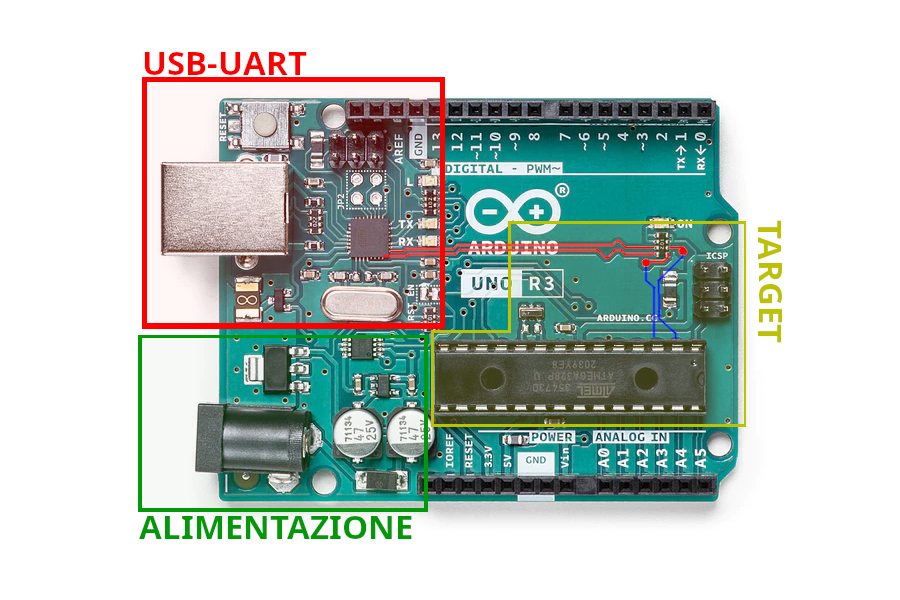
\includegraphics[width=.5\textwidth]{arduino-uno.png}
    \caption[]{Foto di una scheda Arduino Uno R3\cite{img:arduino-uno-r3}}\label{fig:arduino-uno-r3}
\end{figure}

La scheda (Figura~\ref{fig:arduino-uno-r3}) presenta una serie di connettori posti ai lati, collegati direttamente ai pin del controllore principale in posizione centrale, utili per l'interconnessione del dispositivo con i circuiti in sviluppo.
L'hardware addizionale presente sul lato sinistro, invece, permette di alimentare la scheda da una sorgente esterna non regolata tramite il connettore cilindrico nero e di collegare il controllore principale a un computer mediante la porta USB presente in alto a sinistra la quale consente una connessione seriale.
È inoltre possibile effettuare il reset manuale del target tramite il pulsante presente vicino alla presa USB.\@

Il controllore presente al centro della scheda, in un involucro DIP-28\footnote{Dual in-line package, 28 pin}, è un ATMega328P-PU\cite{site:arduino-uno-doc}. La scelta di un involucro ingombrante, in controtendenza con i processi di miniaturizzazione dell'industria elettronica, è causata dal fatto che, per mantenere una dinamica ``\textit{user friendly}'', rende possibile sostituire il controllore in caso di guasto in modo semplice --- essendo il controllore locato in uno zoccolo invece che essere saldato direttamente sulla scheda --- permettendo così di non dover cestinare l'intera scheda elettronica.\cite{site:arduino-uno-doc}

\section{La famiglia AVR}

Il controllore ATMega328P-PU presente sulla scheda di sviluppo è un membro della famiglia AVR di Atmel\cite[1]{avr:m328p}.

Come è possibile identificare dalla figura~\ref{fig:avr-arch} l'architettura del processore della famiglia AVR è di tipo Harvard: è evidente la dicotomia tra memoria del programma (nell'immagine ``\textit{Flash Program Memory}'') e SRAM\cite{harvard-arch}. Questa suddivisione consente di ottimizzare separatamente le due diverse tecnologie di storge intrinsecamente diverse.

È possibile osservare che la grandezza del bus dati è di 8 bit: conseguentemente è possibile dedurre che l'intera architettura si basa sull'unità fondamentale del byte.

Essendo un processore a singolo ciclo vi è poi la totale assenza di \textit{pipelining}. La maggior parte delle istruzioni, infatti, viene eseguita in un solo ciclo di clock\cite[sec 7.6]{avr:m328p} ad esclusione delle operazioni sulle memorie le quali ``stallano'' il processore per questioni di tempi di accesso/scrittura o di istruzioni che coinvolgono dati di lunghezza maggiore di 8 bit, le quali necessitano di essere salvate in più locazioni di memoria flash e quindi risulta necessario il caricamento di più indirizzi per la loro esecuzione.

\begin{figure}[t]
    \centering
    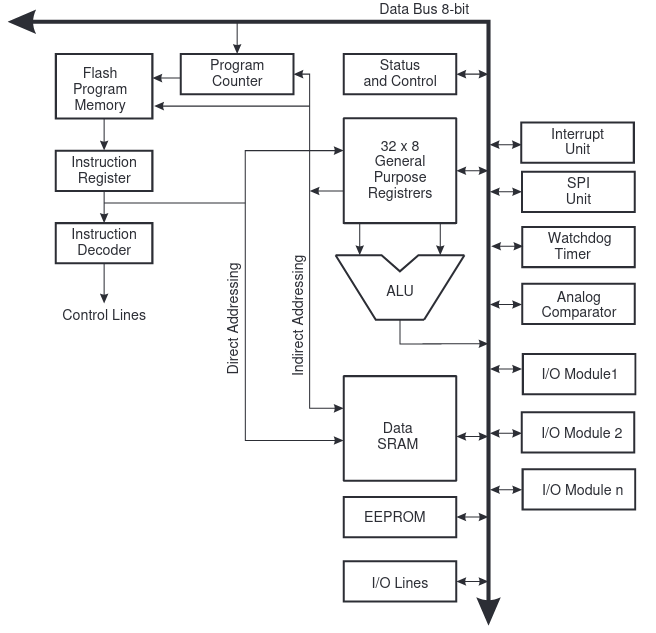
\includegraphics[width=.9\textwidth]{avr_arch.png}
    \caption[Immagine ottenuta dal documento~\cite{avr:m328p} fig 7-1]{Schema a blocchi dell'architettura AVR\cite[fig 7-1]{avr:m328p}}\label{fig:avr-arch}
\end{figure}

\subsection{Funzionalità avanzate}\label{ss:advanced-features}

Per i micro controllori di fascia media esiste la differenziazione tra codice di bootloader e codice eseguibile.

Il codice ``privilegiato'', il bootloader, può essere eseguito se si verificano determinati eventi rilevabili dall'hardware quali condizioni di reset particolari o al verificarsi di una condizione sullo stato di un pin; oppure può essere protetto da sovrascrittura/lettura con criteri diversi dal codice dell'applicazione ed è in grado di riprogrammare la memoria dello stesso integrato mentre è in esecuzione (Read While Write)\cite[sec 27.4]{avr:m328p}. Al contrario, il codice applicativo è destinato alla sola esecuzione.

\subsection{Memorie}

All'interno di un controllore della famiglia AVR, essendo un processore ad architettura harvard, è possibile trovare due diverse tipologie di memorie dedicate --- utili all'ottimizzazione di costi e funzionamento --- e una terza tipologia dedicata all'utilità e alla riduzione dei costi dell'hardware (EEPROM).

\subsubsection{Memoria FLASH}
La memoria flash è dedicata alla conservazione del codice eseguibile.
Dato l'utilizzo generale di sola lettura, essa si presenta come una memoria a lettura veloce, organizzata ad unità elementari di 16 bit --- dimensione minima degli opcode\cite{avr:isa} --- e riprogrammabile a pagine.

Si tratta poi di una memoria complessa: per i controllori avanzati, aventi il supporto al bootloader, essa è divisa in due sezioni le quali garantiscono la possibilità di differenziare i privilegi del codice presente nelle due sezioni come descritto nella sezione~\ref{ss:advanced-features}.

Essendo inoltre una memoria ``di programma'', essa non richiede prestazioni notevoli in scrittura: questa avviene, come detto precedentemente, a pagine, ossia a blocchi di 512/1024 bit (in funzione del controllore e della dimensione della memoria) e può essere eseguita in tre diverse modalità:

\begin{itemize}
    \item ISP\footnote{In System Programming}: In questo caso il controllore è in modalità di programmazione ed esegue i comandi inoltrati da un programmatore esterno --- connesso tramite SPI\footnote{Serial Peripheral Interface} --- mentre la CPU è in stato di \textit{halt}.
    \item Self Programming: Grazie all'istruzione \texttt{spm} è possibile riprogrammare le pagine della memoria flash dall'interno del codice stesso\footnote{Nel caso in cui sia presente il supporto al bootloader, \texttt{spm} può essere eseguito solo se il program counter punta a tale regione.}.
    \item High Voltage Parallel Programming: Viene utilizzato in caso non sia disponibile la linea di reset perché configurata come funzionalità ausiliaria: consiste nell'applicare +12V sulla linea di reset per forzare la programmazione\cite[sec 28.6]{avr:m328p}.
\end{itemize}

\subsubsection{EEPROM}

La memoria EEPROM\footnote{Electrically Erasable and Programmable Read-Only Memory} è considerata una memoria di utilità in quanto non necessariamente essenziale alla vita del codice in esecuzione. Essa permette di salvare dati in modo non volatile nell'eventualità di una mancanza di alimentazione.

Si tratta di una memoria ``lenta'' (tempi di programmazione di 3.4ms\cite[tab 8-1]{avr:m328p}) ma in grado di essere letta e scritta con un'unità fondamentale di 8 bit\cite[sec 8.4]{avr:m328p}.

Il vantaggio che si presenta con l'integrazione di tale memoria all'interno dell'micro-controllore consiste nell'eliminazione di un ulteriore componente sul circuito stampato nel caso essa sia necessaria, oltre al non utilizzo di una periferica di comunicazione dedicata a tale scopo.

L'interazione con la memoria avviene tramite la scrittura e lettura dei registri \texttt{EECR} \texttt{EEDR} \texttt{EEAR} (EEPROM Control, Data e Address Registers)\cite[34]{avr:m328p}.

\subsubsection{SRAM}
La memoria SRAM\footnote{Static Random Access Memory} è uno dei componenti di maggiore importanza della struttura dell'integrato.

Essa consiste nella principale memoria di elaborazione, ma la sua struttura è leggermente più complessa rispetto a quanto si possa trovare su un comune calcolatore.
Infatti l'architettura AVR utilizza in modo marcato il concetto di MMIO\footnote{Memory Mapped Input and Output}.

\begin{figure}[b]
    \centering
    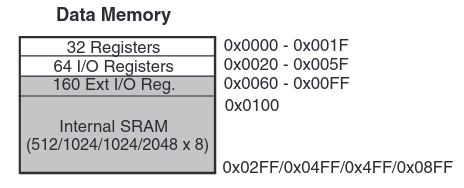
\includegraphics[width=.7\textwidth]{avr_sram_allocation.png}
    \caption[Immagine ottenuta dal documento~\cite{avr:m328p}, fig. 8-3]{Settorizzazione della memoria SRAM del controllore ATMega328P\cite[fig 8-3]{avr:m328p}}\label{fig:avr-sram-alloc}
\end{figure}

Come è possibile osservare dalla figura~\ref{fig:avr-sram-alloc} i primi 128 byte della memoria SRAM sono in realtà registri di uso generale (\texttt{r0}-\texttt{r31}) o registri di controllo delle periferiche.
La scrittura di tali locazioni di memoria causa effetti collaterali in funzione della periferica alla quale è associata. Questa sezione si divide in tre blocchi: i primi 32 byte sono i registri \textit{general purpose} i quali sono interconnessi e interagiscono con l'ALU.\@ Essi vengono utilizzati per l'elaborazione e il salvataggio di dati temporanei.

A seguire sono presenti due zone di memoria: \textit{I/O} ed \textit{Extended I/O} contenenti i registri di controllo delle periferiche. A tal fine, dato che le scritture e le letture possono causare cambiamenti alla periferica (e.g.\ la lettura di un flag \textit{busy} per attendere il completamento di un'operazione prima di eseguirne una seconda) questi indirizzi vengono dichiarati mediante la keyword \texttt{volatile}\footnote{Keyword del compilatore C per impedire l'ottimizzazione delle letture e scritture ad un dato indirizzo}. La differenza tra le due sezioni consiste nella possibilità della prima di essere acceduta in un solo ciclo di clock tramite le istruzioni di \textit{I/O} \texttt{in}, \texttt{out}, ecc\ldots

È possibile notare dalla figura~\ref{fig:avr-sram-timings} come le istruzioni di accesso alla ram impieghino due cicli di clock: l'indicizzazione della ram è effettuata tramite un indirizzamento di 16 bit, il quale rende necessario l'utilizzo congiunto di due registri (r26-r27, r28-r29, r30-r31). 

Questa operazione necessita Il calcolo l'indirizzo al quale effettuare l'operazione incrementando, decrementando oppure lasciando invariata la coppia di registri di indicizzazione pre o post esecuzione. Una volta che l'indirizzo è pronto, esso deve diventare valido prima di poter effettuare l'operazione.

\begin{figure}[t]
    \centering
    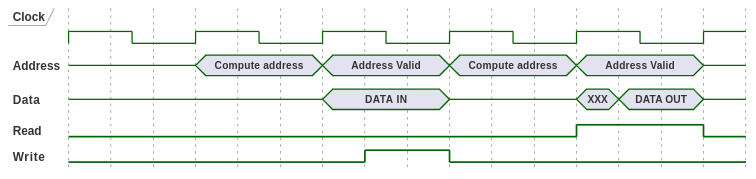
\includegraphics[width=.9\textwidth]{sram-access-timings.png}
    \caption[Immagine rielaborata a partire dalla fig. 8-4 del documento~\cite{avr:m328p}]{Sequenze di accesso in lettura e scrittura della memoria SRAM\cite[fig 8-4]{avr:m328p}}\label{fig:avr-sram-timings}
\end{figure}



\noindent\begin{minipage}{\textwidth}
    \begin{lstlisting}[language=AVR, caption={Esempio di utilizzo dell'istruzione \texttt{st}}, label=lst:store-example]
        ldi r24, 0xFF ;Salva la costante 0xFF nel registro r24
        eor r0, r0 ;Salva la costante 0x00 nel registro r0
        eor r26, r26 ;Azzera il contenuto di r26 (XL)
        eor r27, r27 ;Azzera il contenuto di r27 (XH)
    loop:
        st r24, X+ ;SRAM[r27:r26] = r24
        dec r24 ;r24--
        cpse r24, r0 ;if(r24 == 0) goto hold
        rjmp loop ;else goto loop
    hold:
        rjmp hold ;goto hold

    \end{lstlisting}
\end{minipage}

In particolare, un uso comune delle istruzioni di accesso alla memoria viene mostrato dal listato~\ref{lst:store-example}, riga 6.


Il codice presentato dal listato~\ref{lst:store-example}, mostra nelle linee 1-4 l'azzeramento dei registri r0, r26 e r27 (dove gli ultimi due elencati vengono definiti nel codice dal meta-registro X) e in seguito definisce un ciclo dove viene salvato il contenuto di r24 all'indirizzo puntato dal registro X con successivo incremento; segue l'istruzione \texttt{cpse}\footnote{Compare and Skip if Equal} la quale compara rispetto alla costante 0 il valore di r24 una volta decrementato. Nel caso in cui la comparazione risulti veritiera, viene incrementato il program counter di due \textit{word}, terminando quindi l'esecuzione nel ciclo di \textit{hold}.

\section{La scheda}
Come detto ad inizio capitolo, la scheda utilizzata nello sviluppo del sistema è \textit{Arduino Uno R3}.

È possibile notare come nello schema elettronico della scheda (\ref{app:r3-schematic}) siano presenti due distinti componenti principali e tre sezioni funzionali diverse.

\subsection{Circuito di alimentazione}

Il circuito di gestione dell'alimentazione della scheda si occupa di fornire la tensione adeguata al funzionamento dei due micro-controllori e di utilizzare la sorgente più adatta.

Le due sorgenti di alimentazione della scheda si identificano nel componente \texttt{X1} e nella porta USB \texttt{X2}. Data la presenza di due possibili sorgenti delle quali la prima presenta un input non regolato --- in quanto il componente \texttt{X1} consiste in una presa di alimentazione cilindrica collegata al pin 3 di un regolatore di tensione con intervallo di funzionamento dell'ingresso da 7V a 20V\cite{onsemi:ncp111750} --- si rende necessario un circuito di selezione mostrato dalla figura~\ref{fig:r3-schematic-pwr-sel-detail}.

\begin{figure}[t]
    \centering
    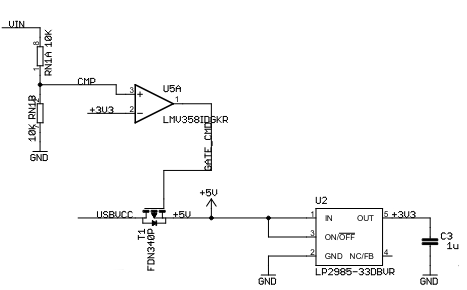
\includegraphics[width=.8\textwidth]{r3-schematic-pwr-sel.png}
    \caption[Dettaglio dello schema elettronico posto in appendice, documento~\ref{app:r3-schematic}]{Dettaglio dello schema elettronico della scheda Arduino Uno R3, documento~\ref{app:r3-schematic}~\cite{site:r3-schematic}}\label{fig:r3-schematic-pwr-sel-detail}.
\end{figure}

Per analizzare il circuito presentato dalla figura~\ref{fig:r3-schematic-pwr-sel-detail} è necessario ipotizzare diversi scenari iniziali.

Ipotizzando il caso in cui la scheda venga collegata ad una sorgente di alimentazione esterna maggiore di 7V tramite il connettore \texttt{X1}, si ha che il collegamento \texttt{USBVCC} avrà tensione pari a 0V.
L'ingresso, inoltre, alimenterà il componente \texttt{U1} (non mostrato in figura) che regolerà la tensione e alimenterà la linea \texttt{+5V}, la quale alimenterà il componente \texttt{U2} che, a sua volta, alimenterà la linea \texttt{+3V3}.
Il comparatore (\texttt{U5A}) avrà uscita a 5V se \texttt{VIN} --- collegato direttamente alla sorgente esterna tramite un diodo (\texttt{D1}) --- è superiore a 6.6V: l'uscita del comparatore pilota il gate del mosfet a canale P \texttt{P1} non avendo però alcun effetto in quanto, come detto precedentemente, \texttt{USBVCC} è posto a 0V.

Ipotizzando ora il caso in cui la scheda è solamente collegata a un computer tramite la porta USB.\@ In questo caso la connessione \texttt{VIN} avrà potenziale 0V.

\texttt{USBVCC} avrà potenziale 5V da specifica USB.\@ In una fase iniziale la linea \texttt{+5V} avrà quindi potenziale pari a 4.3V considerando la caduta di tensione del diodo presente all'interno del componente \texttt{T1}; tensione sufficiente ad alimentare il comparatore \texttt{U5A} e il regolatore di tensione \texttt{U2}.
Essendo \texttt{VIN} posta a 0V, l'uscita del comparatore sarà anch'essa posta a 0V --- essendo il componente LMV358 un amplificatore operazionale \textit{rail-to-rail}\cite{ti:lmv358} ---
stabilendo una differenza di potenziale tra il gate e il source di 5V abbattendo così la resistenza equivalente e portando la linea di alimentazione a 5V effettivi\cite{onsemi:fdn340p}.

Ipotizzando infine che, data la condizione stabile precedentemente descritta, l'utente colleghi la scheda a una seconda sorgente (tramite \texttt{X1}) contemporaneamente all'alimentazione USB.\@ In questo caso, se la tensione VIN è superiore a 6.6V, l'uscita del comparatore \texttt{U5A} incrementerà a 5V, causando così una differenza di potenziale gate-source per il componente \texttt{T1} di 0V e di conseguenza la ``disconnessione'' del carico da \texttt{USBVCC}.

\subsection{Comunicazione con l'host}

Il caricamento e la comunicazione tra \textit{target} e \textit{Host} avvengono tramite una linea seriale UART.\@ Ne consegue il problema di adattare un'interfaccia seriale TTL non presente su un computer \textit{consumer grade} a una presente sulle comuni piattaforme di elaborazione.

Questa funzionalità viene svolta dal componente \texttt{U3} dello schema allegato (\ref{app:r3-schematic}). Esso è un microcontrollore della famiglia AVR con il supporto USB.\@

In particolare si tratta di un \texttt{ATMega16U2} con caricato un firmware che implementa la classe CDC del protocollo USB, rendendo il dispositivo una periferica RS232 virtuale.
Il firmware si occupa di ricevere i dati dall'\textit{host} e di replicarli sulla linea seriale (pin 8 e 9) e vice versa.\cite[firmwares/atmegaxxu2/arduino-usbserial/]{git:arduinocore}.

\begin{figure}[t]
    \centering
    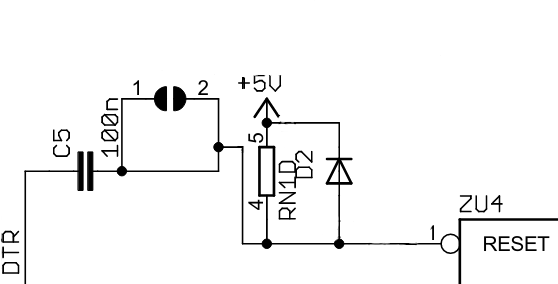
\includegraphics[width=.8\textwidth]{r3-rst-cap.png}
    \caption[Dettaglio dello schema elettronico posto in appendice, documento~\ref{app:r3-schematic}]{Dettaglio della connessione alla linea di reset dell'ATMega16U2, documento \ref{app:r3-schematic}~\cite{site:r3-schematic}}\label{fig:r3-schematic-rst-detail}.
\end{figure}


Oltre alle connessioni relative alla comunicazione seriale tra \textit{target} e ATMega16U2 è presente una terza connessione che pilota la linea di reset del primo. Il pin 13 dell'ATMega16U2 è connesso, tramite \texttt{C5} alla linea di reset del \textit{target}.

Secondo la specifica RS-232, oltre alle due linee seriali (TXD e RXD), sono presenti anche delle line di ``\textit{flow control}'', tra le quali possiamo notare la linea \texttt{DTR}.

Questa linea è asserita dalla maggior parte dei driver seriali (e seriali virtuali) al momento della connessione al dispositivo o del collegamento. Così facendo, grazie a \texttt{C5} è possibile avere un impulso sulla linea di reset prima che il circuito ritorni all'equilibrio: Inizialmente il condensatore \texttt{C5} si trova in equilibrio con la linea DTR posta a 5V e la linea di RESET posta a +5V per mezzo della resistenza di pull'up. Al momento dell'asserzione, la linea DTR viene posta a 0V: il condensatore \texttt{C5} si carica causando un calo nella linea di reset fino a 0V, la quale poi evolverà secondo il modo del sistema dato dal prodotto tra la resistenza e la capacità di \texttt{RN1D} e \texttt{C5}.
Al momento della disconnessione il condensatore causerà un picco positivo nella linea di reset fino a circa 10V che viene però soppresso dalla presenza di \texttt{D2}.

\subsection{Programmazione}

La programmazione dell'integrato \textit{target} non avviene secondo i metodi tradizionali ma attraverso un bootloader pre-caricato\cite[bootloaders/atmega/ATmegaBOOT\_168.c]{git:arduinocore}. 
Una volta forzato il reset tramite l'asserzione della linea \texttt{DTR} il bootloader viene attivato e, in caso di ricezione di comandi di programmazione, esso inizia la programmazione tramite l'istruzione \texttt{spm}.

    \chapter{Architettura di sistema}

Affinché l'utente sia agevolato nello sviluppo di un firmware, egli deve sfruttare al meglio l'interoperabilità dei componenti e le potenzialità dell'intero sistema di sviluppo.

Risulta quindi necessaria una visione di insieme dell'intero sistema invece che una valutazione locale dei singoli componenti in parallelo a una valutazione della compatibilità inter-componente affinché la loro interazione permetta allo sviluppatore di operare con facilità.

\begin{figure}[t]
    \centering
    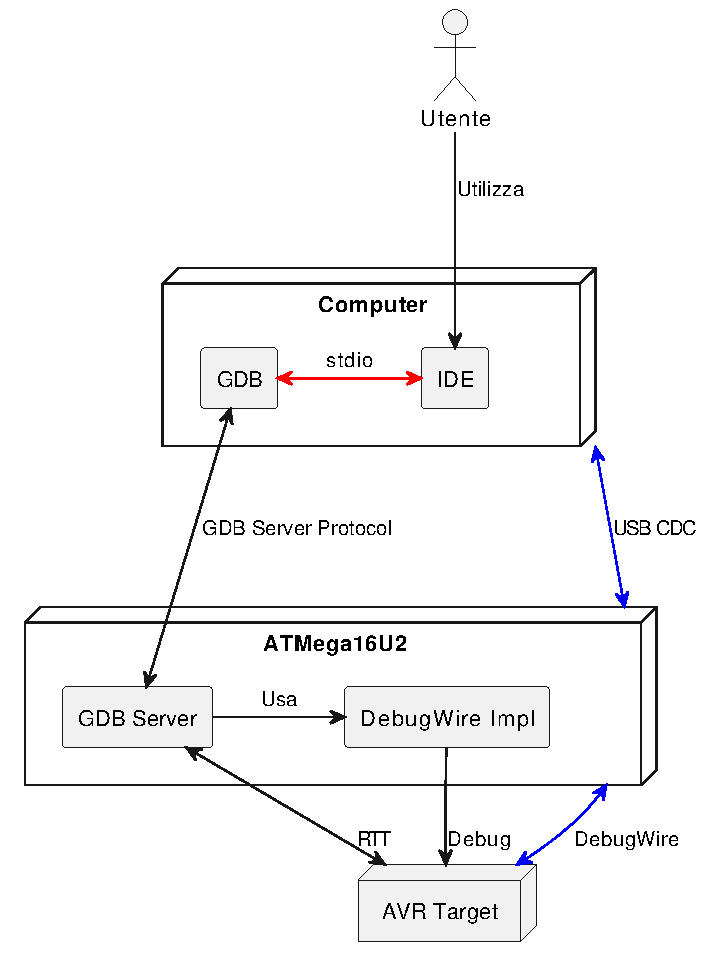
\includegraphics[width=.7\textwidth]{sys-arch.pdf}
    \caption[]{Diagramma dei componenti del sistema di assistenza alla programmazione e debugging}\label{fig:sys-arch}
\end{figure}

Come osservabile dalla \cref{fig:sys-arch}, il sistema sviluppato si basa su tre livelli fisici collegati a cascata da protocolli (indicati in blu nella figura), in modo tale da adattare le azioni ad alto livello scelte dall'utente ai comandi di debug a basso livello che permettono di interagire con il controllore \textit{target}. 

Il primo livello, ovvero il livello di interfaccia con lo sviluppatore, consiste nel software utilizzato per lo sviluppo del firmware contenente tutti gli strumenti di supporto alla programmazione C. Questi software, anche noti come IDE\footnote{Integrated Development Environment}, hanno il compito di accorpare svariate funzionalità mediante integrazione di software esterni allo scopo di favorire lo sviluppo fornendo un ambiente unico e integrato allo sviluppatore, dal quale effettuare tutte le operazioni quali sviluppo, compilazione, debugging e upload.

Enfasi particolare viene posta sull'integrazione da parte dell'IDE del software GDB, il quale svolge il compito di processo \textit{debugger}, ovvero il processo responsabile della gestione delle richieste al server di debug per controllare il comportamento e il flusso di esecuzione di un processo \textit{target} nominato ``processo \textit{debuggee}''.

Il \textit{debugging} è una delle pratiche ormai fondamentali della programmazione che permette una comprensione agevolata del flusso di esecuzione del codice e permette di ispezionarne i vari stati.

In particolare esso garantisce la possibilità di analizzare uno stato intermedio tramite l'esecuzione del codice in modo interattivo, consentendo allo sviluppatore di condurre ``un'indagine'' relativa a un funzionamento inatteso del firmware. Per citare un detto diffuso sulle piattaforme social in ambito di programmazione possiamo affermare che la procedura di \textit{debugging} sia paragonabile ad un'indagine condotta dallo sviluppatore dove egli stesso è il colpevole.

È necessario porre un'ulteriore enfasi sull'aggettivo ``interattivo'': la differenza tra \textit{debugging} e \textit{logging} sta proprio nel fatto che il secondo consiste solamente nella stampa, su un terminale o file, di una serie di messaggi statici e predefiniti al fine di tracciare gli eventi per un'analisi futura e inaspettata. Ciò non permette quindi di effettuare decisioni in funzione dei risultati parziali ottenuti nella procedura di \textit{debugging} a meno di riprogrammare il dispositivo --- inficiando così la longevità delle memorie --- e ricapitolare l'esecuzione del codice.

Risulta quindi di grande importanza poter accedere a uno (o più) software per il debugging in modo che esso possa essere efficiente.
Uno dei software più utilizzati per il debugging del codice compilato, qualunque sia il linguaggio scelto, è Gnu GDB\cite{site:gdb}.

\section{Gnu Debugger}\label{sec:gdb}

Il software GDB è un debugger multiarchitettura\cite{site:gdb} utilizzato per l'ispezione degli stati di esecuzione dei software compilati.
In particolare esso presenta un'architettura multipla di funzionamento in funzione della localizzazione del processo da ispezionare.

Generalmente il processo da analizzare è direttamente localizzato sulla stessa macchina nella quale il processo GDB viene istanziato. In questo caso è sufficiente utilizzare delle chiamate di sistema (\textit{syscall}) in grado di accedere e bloccare l'esecuzione del processo da parte del sistema operativo.
Sarà dunque possibile modificare il contenuto della porzione di memoria in cui è caricato l'eseguibile in modo da sostituire l'istruzione incriminata con un'istruzione di ``\textit{break}''. Questa istruzione causerà, al momento della sua esecuzione, un'eccezione a livello hardware la quale verrà gestita dal kernel e notificherà il processo \textit{debugger} che il processo \textit{debuggee} ha raggiunto un \textit{breakpoint}.

Purtroppo non sempre il processo \textit{debuggee} è in esecuzione sullo stesso processore in cui si trova il processo GDB client. Questo comporta la necessità di scindere in due componenti il programma utilizzato per effettuare il \textit{debug} adottando un'architettura client-server per consentire la dislocazione del processo \textit{debuggee}.

\subsection{Debugging di dispositivi embedded}

Quanto enunciato precedentemente si avvera nel debugging di dispositivi embedded. 

Possiamo vedere il firmware in esecuzione sul microcontrollore come un processo dislocato su un processore remoto con una diversa architettura.

La problematica relativa alla diversa architettura dei processori non costituisce motivo di preoccupazione in quanto ormai la maggior parte degli \textit{instruction set} è stata inclusa nella distribuzione di GDB multi-architettura\cite{site:gdb}.
La vera problematica si ha con la scarsa connettività dell'integrato, la quale richiede un protocollo e un componente di adattamento \textit{ad-hoc}.
L'architettura client-server permette quindi di implementare tale adattatore su un dispositivo esterno connesso con il \textit{target} con possibilità di implementare il protocollo di debug permettendo così di adattare l'interfaccia a tutti i dispositivi in grado di eseguire GDB.\@ 

Possiamo vedere come la concezione di separazione tra applicativo di controllo e interazione ed esecutore dei comandi di debug può essere implementata dalla \cref{fig:gdb-server-tunnels}.

\begin{figure}
    \centering
    \begin{tikzpicture}
        \draw[fill=green!50] (0,3) rectangle (4,4) node[pos=.5] {GDB}; %GDB
        \draw[fill=yellow!50] (0,2) rectangle (4,3) node[pos=.5] {GDB proto}; %gdb_proto
        \draw[fill=red!50] (0,1) rectangle (4,2) node[pos=.5] {CDC}; %cdc
        \draw[fill=blue!50] (0,0) rectangle (4,1) node[pos=.5] {USB PHY}; %usb_phy
        
        \draw[fill=purple!50,purple!50,text=black] (5,3) rectangle (9,4) node[pos=.5] {GDB server}; %GDB_SERVER
        \draw[fill=purple!50,purple!50] (7.5,2) rectangle (9,3); 
        \draw (5,3) -- (5,4) -- (9,4) -- (9,2);

        \draw[fill=yellow!50] (5,2) rectangle (7.5,3) node[pos=.5] {GDB proto}; %gdb_proto
        \draw[fill=red!50] (5,1) rectangle (7.5,2) node[pos=.5] {CDC}; %cdc
        \draw[fill=blue!50] (5,0) rectangle (7.5,1) node[pos=.5] {USB PHY}; %usb_phy
        \draw[fill=gray!50] (7.5,1) rectangle (9,2) node[pos=.5] {dW}; %dw
        \draw[fill=orange!50] (7.5,0) rectangle (9,1) node[pos=.5] {UART}; %uart

        \draw[fill=cyan!50] (10,2) rectangle (14,3) node[pos=.5] {Target Process}; %AVR
        \draw[fill=gray!50] (10,1) rectangle (14,2) node[pos=.5] {dW}; %dw
        \draw[fill=orange!50] (10,0) rectangle (14,1) node[pos=.5] {UART (O.D.)}; %UART

        \draw[black, thick] (2, 0) -- (2, -0.5) -- (6.25, -0.5) -- (6.25, 0);
        \draw[black, thick] (8.5,0) -- (8.5, -0.5) -- (12, -0.5) -- (12, 0);

        \node (5) at (2, 4.5) {Host};
        \node (5) at (7, 4.5) {Adapter};
        \node (5) at (12, 4.5) {Tagret (AVR)};
    \end{tikzpicture}
    \caption[]{Diagramma di incapsulamento e protocolli di comunicazione tra debugger e target}\label{fig:gdb-server-tunnels}
\end{figure}

In particolare, la figura rappresenta la scelta intrapresa per lo sviluppo del sistema in esame. È possibile notare come il software GDB si interfacci al relativo server presente sull'adattatore (firmware presente sull'ATMega16U2) tramite il protocollo GDB appoggiandosi al protocollo USB-CDC per l'invio dei pacchetti di comunicazione e venga trasmesso sul bus seriale differenziale.
Questi pacchetti vengono quindi convertiti dal server precedentemente menzionato il quale esegue le azioni richieste sul \textit{target} tramite la connessione DebugWire.

\subsection{Integrazione con ambienti di sviluppo}\label{ss:code-decoration}

L'integrazione con gli ambienti di sviluppo avviene sfruttando la standardizzazione dei comandi che GDB definisce. Siccome GDB implementa un'interfaccia da linea di comando dove tutti gli input e output sono ben definiti secondo uno standard, risulta di facile implementazione un software in grado di dialogare con il \textit{debugger} il cui fine è di introdurre un'interfaccia grafica per agevolare lo sviluppatore. Inoltre le informazioni tratte dallo stream (stdin/stdout) possono essere mostrate in modo effettivo nell'IDE andando a decorare il codice, ovvero ad aggiungere informazioni ``tra le righe'' permettendo allo sviluppatore di focalizzarsi sullo sviluppo come da \cref{fig:vscode-dbg-dec}.

\begin{figure}[t]
    \centering
    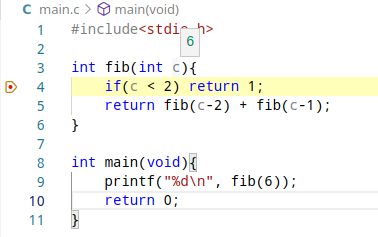
\includegraphics[width=0.8\textwidth]{vscode-dbg-decoration.png}
    \caption[]{Esempio di decorazione del codice durante il debug.}\label{fig:vscode-dbg-dec}
\end{figure}

\section{GDB Server e Livello fisico}

Il secondo livello è costituito dal firmware presente sull'ATMega16U2 collocato sulla scheda \textit{Arduino Uno R3} (componente \texttt{U3}).

Questo firmare, completamente ripensato rispetto all'originale, si occupa di convertire i comandi inviati dall'\textit{host} tramite una connessione USB simulando un dispositivo seriale e di adattarli al debugging tramite DebugWire, implementando un server GDB direttamente all'interno dell'integrato.

Il secondo livello si occuperà di mantenere una connessione compresa di stato con il \textit{debugger}, ``tradurre'' i comandi GDB in modo che possano essere inoltrati al target tramite protocollo DebugWire e garantire funzionalità aggiuntive quali un livello di comunicazione \textit{target-to-host} su connessione di debug nominato Real Time Terminal (RTT).

Il firmware dell'ATMega16U2 è composto da quattro macro regioni descritte a seguire in questa relazione:
\begin{enumerate}
    \item Comunicazione USB con l'\textit{host}, implementata grazie all'utilizzo di una libreria esterna (LUFA\footnote{https://github.com/abcminiuser/lufa}).
    \item Server GDB
    \item Implementazione dell'interfaccia seriale open collector
    \item Implementazione del protocollo DebugWire
\end{enumerate}

\subsection{Protocollo GDB}

Il protocollo per la comunicazione client-server di GDB è definito a partire da un canale di comunicazione in grado di trasmettere caratteri \textit{ASCII}.
Così facendo è possibile trasmettere anche su canali strettamente testuali e non standard (simboli da 7 bit).

Affinché sia possibile trasmettere dati in tale formato è necessario ricorrere alla codifica esadecimale testuale dei numeri come definita dai \cref{lst:nib-2-char,lst:char-2-nib} i quali rappresentano due funzioni di conversione da intero a esadecimale testuale e viceversa.
Si noti come nelle funzioni si parli di \textit{nibble}, ovvero un'unità di quattro bit (che possono prendere valori compresi tra 0 e 15). Questo perché un byte viene convertito in due caratteri alfabetici per essere rappresentato in esadecimale e, similmente, due caratteri alfabetici rappresentano un solo byte.

\noindent\begin{minipage}{\textwidth}
    \begin{lstlisting}[style=C, caption={Funzione di conversione da nibble a carattere alfabetico}, label=lst:nib-2-char]
    char nib2hex(unsigned char nib){
        /*
            Se il valore da mappare è minore di dieci allora sarà una cifra
        */
        if(nib < 10) return nib + '0'; 

        /*
            Altrimenti sarà una lettera (minuscola)
        */
        return nib - 10 + 'a';
    }
    \end{lstlisting}
\end{minipage}

\noindent\begin{minipage}{\textwidth}
    \begin{lstlisting}[style=C, caption={Funzione di conversione da carattere alfabetico a nibble}, label=lst:char-2-nib]
    unsigned char hex2nib(char hex){
        /*
            Se il valore è una cifra allora ricaviamo l'offset dalla cifra `0' in quanto sequenziali
        */
        if(hex >= '0' && hex <= '9') return hex - '0';
        /*
            Altrimenti riproponiamo per la lettera 'a' + 10
        */
        return hex - 'a' + 10;
    }
    \end{lstlisting}
\end{minipage}

I valori stabiliti negli offset sono di facile interpretazione: si ricordi che nel linguaggio C i caratteri hanno lo stesso significato di interi a otto bit, di conseguenza è possibile sommare o sottrarre caratteri i quali verranno interpretati con il loro relativo valore numerico assegnato dalla tabella \textit{ASCII}. 

In particolare il carattere `a' corrisponde al valore esadecimale 0x41 e il carattere `0' corrisponde al valore 0x30. Si ricordi che le cifre numeriche e le lettere, siano esse minuscole o minuscole, sono sequenziali in tale tabella.

Il protocollo GDB, inoltre, permette al server --- quando il target non è in stato di \textit{halt} --- di inviare notifiche da mostrare a schermo mediante il comando \texttt{O}.

Questa funzionalità sarà la base per l'implementazione del terminale in tempo reale.

\subsubsection{Formato}

I pacchetti inviati sul canale di comunicazione, come mostrato dalla \cref{fig:gdb-packet}, sono composti da una sezione contenente il comando e delimitata dai caratteri \texttt{\$} e \texttt{\#} seguita da due caratteri esadecimali rappresentanti un byte di controllo il cui valore è dato dall'\cref{eq:gdb-checksum}

\begin{figure}[t]
    \centering
    \begin{bytefield}[endianness=big,bitwidth=1em]{32}
        \bitbox{4}{\$} & \bitbox{20}{cmd} & \bitbox{4}{\#} & \bitbox{4}{CHKSM}\\
    \end{bytefield}
    \caption[]{Struttura di un pacchetto utilizzato nella comunicazione client-server GDB.}\label{fig:gdb-packet}
\end{figure}

\begin{equation}\label{eq:gdb-checksum}
    CHKSM = byte2asciihex \left( \sum_{1=0}^{\# cmd} \left(cmd_i\right) \ \bmod{256}\right)
\end{equation}

Questa procedura permette di implementare un parser di comandi a bassissimo impatto sulla memoria RAM in quanto è possibile calcolare il \textit{checksum} durante la ricezione.

Il formato dei comandi è generalmente definito come una lettera alfabetica seguita da una serie di parametri separati dal carattere virgola e a seguire gli argomenti, codificati in esadecimale alfabetico, separati dai parametri tramite i due punti\cite{site:gdbproto}.
    \chapter{DebugWire}
\section{Descrizione del protocollo e fondamentali}

Parte fondamentale del core AVR, omessa dal diagramma in figura~\ref{fig:avr-arch}, è il sistema di \textit{debugging} on chip ``\textit{DebugWire}''.

Esso permette, tramite un tool esterno collegato all'integrato, di stallare la cpu e leggere e scrivere le memorie e i registri.\cite[sec 25]{avr:m328p}

Affinché le funzionalità di debugging siano disponibili, è necessario abilitare la periferica DebugWire tramite i bit di configurazione al momento della programmazione del dispositivo\cite[tab 28-7]{avr:m328p}.

\subsection{Interfaccia fisica}\label{ss:dw-phy}

L'interfacciamento fisico tra controllore e dispositivo esterno avviene tramite una sola connessione al pin di reset dell'integrato \textit{target}.

Il fatto che l'interfaccia di debug sia collocata sul pin di reset comporta che, una volta abilitata la periferica DebugWire, non sia più possibile resettare il dispositivo o programmarlo tramite interfaccia ISP\cites{avr:appnote:isp}[sec 25.3]{avr:m328p}, ma si rende necessaria una procedura di disattivazione temporanea o la possibilità di programmare l'integrato tramite il protocollo DebugWire.

La comunicazione tra programmatore e target è di tipo seriale e half duplex data la natura della connessione. In particolare il protocollo utilizzato è una derivazione di una seriale UART su un bus open collector, come è osservabile dalla figura~\ref{fig:dw-schematic}\cite{site:dw-reverse-engeneering}.

\begin{figure}[t]
    \centering
    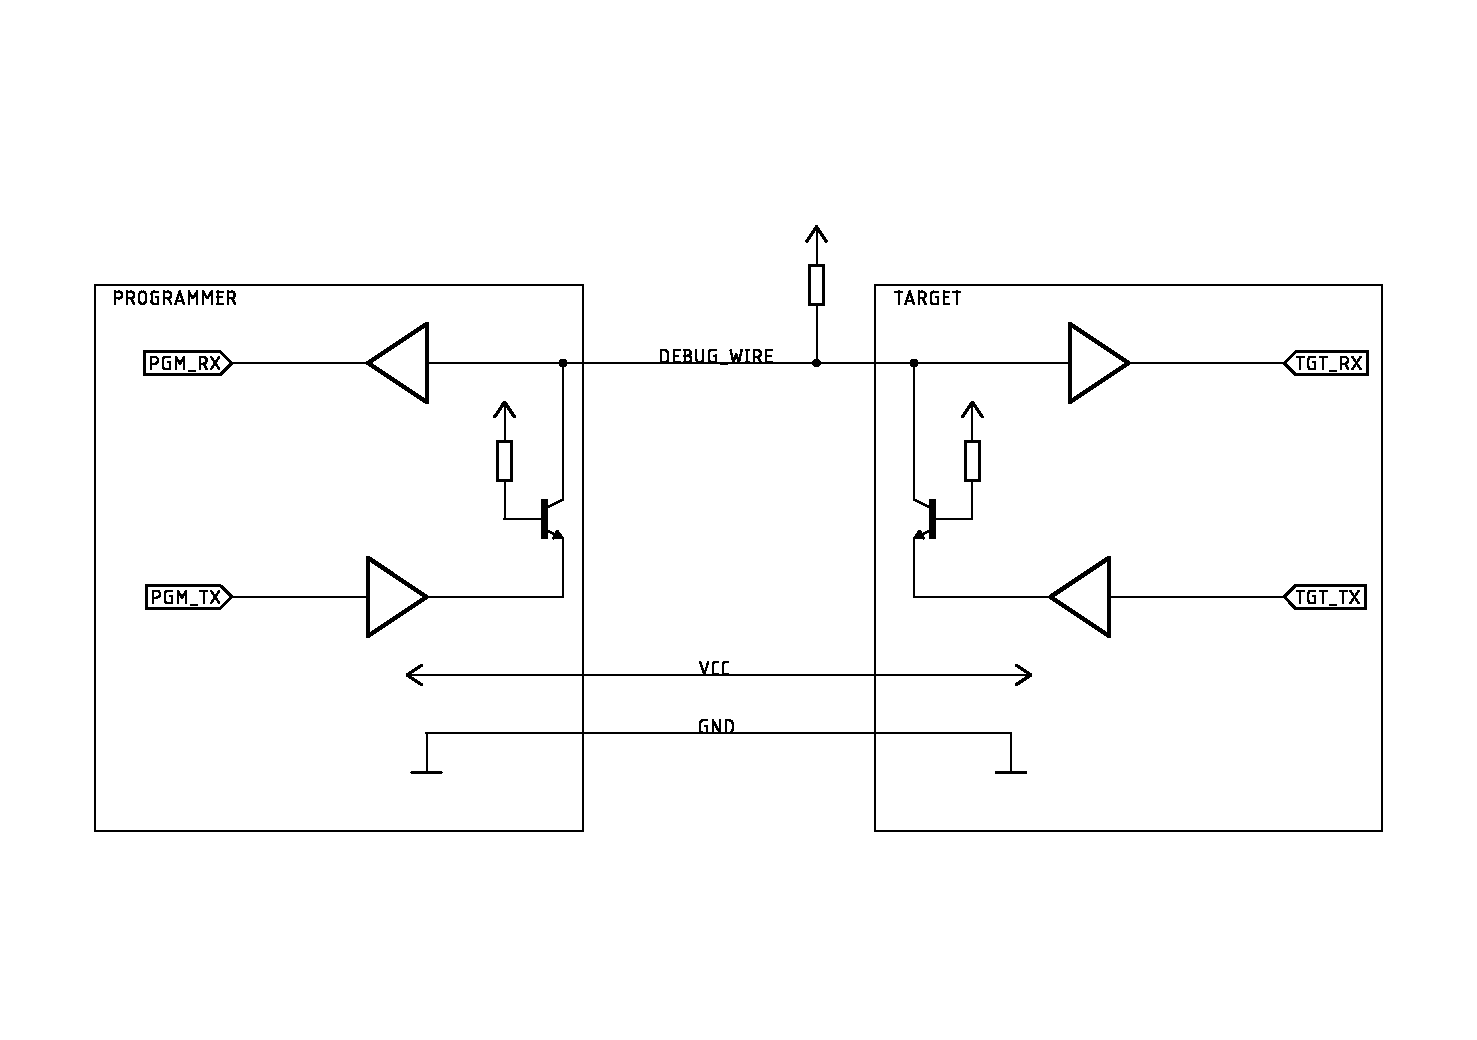
\includegraphics[width=\textwidth]{dw-schematic.pdf}
    \caption[]{Schema concettuale del funzionamento dell'interconnessione tra programmatore e controllore target per il protocollo DebugWire}\label{fig:dw-schematic}
\end{figure}

\subsubsection{Protocollo UART}

Il protocollo UART è un metodo di trasmissione punto-punto digitale seriale asincrono che generalmente lavora su due connessioni tra i due attori della comunicazione. Le due linee rimangono a livello logico 1 quando non c'è attività.

Le linee prendono il nome di ``TX'' e ``RX'' in funzione dell'utilizzo che la periferica master ne fa: è necessario notare come le due linee vengano ``incrociate'' in modo tale da far sì che il pin di trasmissione di un attore vada a collegarsi con il pin di ricezione della controparte.

Essendo un protocollo asincrono, ovvero vi è assenza di una linea di sincronizzazione (clock), le due parti della comunicazione devono conoscere a priori la velocità e il formato dei dati attesi sulle linee.

La trasmissione inizia con un periodo di livello logico 0 (\textit{Start Bit}), in modo che sia possibile l'identificazione dell'inizio della trasmissione di un simbolo rilevando il fronte di transizione da livello logico 1 a livello logico 0 (\textit{Falling Edge}).

Durante questo tempo di bit dove la linea di trasmissione è a livello logico 0 è dunque possibile inizializzare l'hardware e sincronizzare le sorgenti di clock per la ricezione. In seguito al bit di inizio si susseguono i bit del dato, dal meno significativo al più significativo, con periodo pari al tempo di bit stesso. In funzione della specifica del protocollo possono essere inviate unità di dati fondamentali di dimensione da 5 a 8 bit.

A seguito dei bit di dati viene quindi inviato opzionalmente un bit di parità per garantire l'integrità dei dati e successivamente la linea viene posta a livello logico 1 per uno o due periodi di bit, permettendo al ricevitore di eseguire operazioni e resettare la macchina a stati per la ricezione dell'eventuale simbolo seguente.\cite{site:rs-uart}

Essendo un sistema asincrono è opportuno ipotizzare il disallineamento delle frequenze di invio e campionamento: in tal caso una desincronizzazione può essere tollerata se entro il limite dato dall'equazione~\ref{eq:uart-max-delay}
\begin{equation}\label{eq:uart-max-delay}
    t_{delay_{\max}} = \frac{1}{2}(N_{data}+N_{parity}+N_{stop}+1)t_{bit}    
\end{equation}
dove \(N_{data}\) è il numero di bit contenuti nel simbolo inviato che è stato negoziato, \(N_{parity}\) indica il numero di bit di parità, \(N_{stop}\) il numero di \textit{stop bits} e \(t_{bit}\) è il tempo per bit. Inoltre si tiene conto del bit di inizio (\textit{start bit}). Questo comportamento può essere notato dalla figura~\ref{fig:uart-sync}, dove vengono rappresentati il caso ideale e il caso di desincronizzazione massima. In ogni caso si ha che il campionamento avviene all'interno del bit in invio.

\afterpage{
    \begin{figure}[ht]
        \centering
        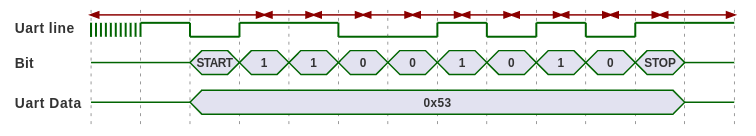
\includegraphics[width=.8\textwidth]{uart-sync.png}\\
        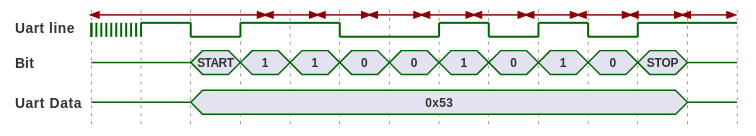
\includegraphics[width=.8\textwidth]{uart-unsync.png}
        \caption[]{I diagrammi di sequenza dimostrano che, anche in caso di non sincronizzazione delle frequenze di invio e ricezione viene mantenuta l'integrità dei dati trasmessi. Viene mostrata una comunicazione seriale 8N1\footnote{Definizione della configurazione di una linea seriale. Essa è composta da tre caratteri: <Numero di bit dati><Tipo di parità ([N]one, [O]dd, [E]ven, [M]ark, [S]pace)><Numero di Stop bits>}}\label{fig:uart-sync}
    \end{figure}
}

La motivazione per cui il campionamento avviene a metà del tempo di bit è data dal fatto che la desincronizzazione può essere causata da una frequenza più alta o più bassa, per cui vale la relazione descritta dall'equazione~\ref{eq:uart-period-receive-delay}
\begin{equation}\label{eq:uart-period-receive-delay}
     t_{bit_{recv}} = t_{bit_{snd}} \pm t_{delay_{\max}}
\end{equation}

Infine, se la velocità di trasmissione fosse misurata in \textit{bit per secondo}, secondo la formula \(v_{uart} = \frac{1}{t_{bit}}\), essa non sarebbe veritiera e porterebbe confusione, in quanto la formula sopra enunciata includa nel conteggio dei bit trasmessi anche i bit di controllo (Start, parity e Stop bit) i quali non contribuiscono all'informazione inviata. Di conseguenza è opportuno definire la velocità di trasmissione della linea seriale come il numero di simboli trasmessi per secondo. Questa definizione differisce dalla prima un quanto il simbolo è composto da un numero di bit non necessariamente pari a 8.

È possibile determinare la velocità in baud a partire dal bitrate e dalla configurazione della linea UART secondo la relazione~\ref{eq:baud-from-bit-rate}\cite{site:baud}:
\begin{equation}\label{eq:baud-from-bit-rate}
    v_{tx_{baud}} = \frac{1}{t_{bit}(N_{data} + N_{parity} + N_{stop} + 1)}
\end{equation}

Da quanto è possibile dedurre dall'equazione~\ref{eq:baud-from-bit-rate}, l'effettivo bit rate di trasmissione della linea UART differisca di un fattore di \(\frac{N_{data}}{N_{data} + N_{parity} + N_{stop} + 1}\) rispetto al bitrate grezzo di trasmissione \(v_{uart}\)

\subsection{Funzionamento}

Tutte le comunicazioni che avvengono sul bus DebugWire non hanno alcun tipo di verifica dell'integrità del dato (Serial 8N1). La comunicazione può avvenire in qualsiasi momento.

In particolare il reset della comunicazione tra target e programmatore/debugger avviene mediante l'invio di un BREAK\footnote{La linea viene posta a livello logico 0 per più di 9 tempi di bit} sulla linea.
Ogni qualvolta sia rilevato un errore (per esempio viene ricevuto un byte inatteso o un comando non noto), il primo attore che rileva l'errore invierà un BREAK che causerà il reset della controparte.

Ciò è possibile perché la connessione è un bus open collector: il conflitto di accesso avviene solo ponendo la linea a livello logico 0 e non comporta cortocircuitazioni di qualsiasi genere. Il conflitto viene rilevato quando un attore legge dal bus uno stato diverso da quanto inviato durante la trasmissione del bit (in particolare quando l'attore riceve un bit pari a 0 quando sta inviando un bit di valore 1).

La velocità di comunicazione è invece definita in funzione della frequenza della cpu del target. Nell'hardware della periferica è presente un \textit{prescaler} (il cui valore di default è di 128) e la velocità di comunicazione viene stabilita come \[v_{com} = \frac{f_{cpu} [Hz]}{prescaler}[bps]\]

Ad ogni reset della comunicazione il prescaler viene resettato al valore iniziale.

In risposta ad un BREAK il target risponderà sempre con l'invio di un valore noto (0x55), facendo sì che a livello fisico sia inviata un'onda quadra con frequenza \(v_{com}\)\cite{site:dw-reverse-engeneering} (si veda figura~\ref{fig:dw-timings})

\begin{figure}[ht]
    \centering
    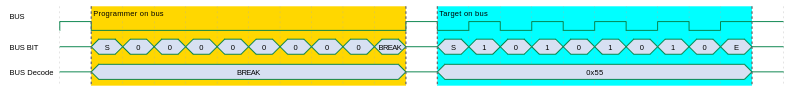
\includegraphics[width=\textwidth]{dw-break-timing.png}
    \caption[]{Diagramma delle tempistiche del bus DebugWire durante il reset della trasmissione}\label{fig:dw-timings}
\end{figure}

È dunque possibile definire un algoritmo per l'inizializzazione della sessione in modo che la frequenza della trasmissione venga dedotta dalla risposta del target invece che essere nota a priori, permettendo un untilizzo semplificato della periferica.

L'algoritmo è strutturato come segue
\begin{enumerate}
    \item Preparazione dell'hardware e inizializzazione strutture dati
    \item Invio di un break dalla durata di 100ms. La durata viene stabilita in funzione della frequenza di trasmissione ragionevolmente più bassa possibile: Considerando che la famiglia AVR integra nei suoi controllori un oscillatore RC a 128kHz usato comunemente per operazioni ``low power'' e ipotizzando che sia abilitata la funzionalità di divisione del clock per un fattore di 8\cite[sec 9.11, tab 28-9]{avr:m328p}, si ottiene una frequenza del core di 16kHz. Ponendo quindi il prescaler di comunicazione DebugWire a 128 otteniamo una frequenza di trasmissione di 125Hz, ovvero 8ms per bit. Infine, sapendo che il tempo di break consiste in almeno 10 bit trasmessi a 0, si ottiene un tempo minimo di break di 80ms, arrotondato a 100ms
    \item Attesa del primo fronte di transizione da livello logico 1 a livello logico 0
    \item Attesa del successivo fronte di transizione da livello logico 0 a livello logico 1 (calcolando il tempo intercorso tra i due fronti)
\end{enumerate}

A questo punto è possibile trovare la frequenza di bit dalla quale ricavare il baud rate.

\subsection{Comandi e features}

Una volta che la cpu del controllore target è in stato \textit{halt} è possibile interagire con la periferica DebugWire per eseguire le operazioni di debug. A seguito di un BREAK e successiva risposta è possibile interpellare il controllore con i comandi descritti di seguito.

Vi sono due classi di comandi: comandi basilari e comandi composti.
I primi sono comandi che svolgono azioni semplici e definite staticamente, quali la scrittura del Program Counter, Instruction register, scrittura del registro di breakpoint hardware e configurazione di flag e comunicazione. Tramite questi comandi è possibile definire i limiti di scrittura/lettura delle memorie e eseguire istruzioni.
I Secondi sono operazioni complesse che necessitano parametri di configurazione i quali sono impostati tramite comandi basilari.

I comandi disponibili per l'interazione con il microcontrollore target tramite DebugWire sono limitati e appartengono a quattro categorie: \textit{Communication Settings}, \textit{Flag Setting},\textit{Program Flow Control} e \textit{Memory R/W}.

\subsubsection{Communication Settings}

Questi comandi vengono utilizzati per modificare il valore del prescaler di comunicazione in modo da variare la velocità di trasmissione. Sono comandi particolarmente utili nel debugging di controllori a bassa frequenza (128kHz).

Non vi è una logica nota nell'assegnazione del comando al corrispondente valore del prescaler: si rende necessaria una tabella di associazione come riportato dalla tabella~\ref{tab:dw-presc-settings}

\begin{table}[ht]
    \centering
    \begin{tabular}{ c c c }
        \textbf{Comando} & \textbf{Valore del prescaler} & \textbf{Bitrate a 16MHz} \\
        \hline
        0x83 & 128 & 125kbps \\
        0x82 & 64 & 254kbps \\
        0x81 & 32 & 500kbps \\
        0x80 & 16 & 1Mbps \\
        0xA0 & 8 & 2Mbps \\
        0xA1 & 4 & 4Mbps \\
        0xA2 & 2 & 8Mbps \\
        0xA3 & 1 & 16Mbps \\
        \hline
    \end{tabular}
    \caption[]{Tabella descrittiva dei comandi per la modifica del prescaler di trasmissione della periferica di debug del controllore target\cite{site:dw-reverse-engeneering}}\label{tab:dw-presc-settings}
\end{table}

Una volta inviato il comando di configurazione del prescaler il controllore si adatterà alla velocità richiesta e risponderà con il valore \texttt{0x55} inviato alla nuova frequenza. Questo valore può essere usato per settare adattivamente la frequenza del programmatore oppure per verificare che le impostazioni siano corrette.

\subsubsection{Flag Setting}

È necessario configurare lo stato della periferica prima di eseguire effettivamente le operazioni che sono state preparate. Possiamo chiamare questo stato ``Contesto di esecuzione'' in quanto la stessa configurazione dell'hardware permette di eseguire diverse azioni in funzione del contesto che viene configurato.

I contesti disponibili sono elencati nella tabella~\ref{tab:dw-contexts}.

\begin{table}[ht]
    \centering
    \begin{tabular}{ c l }
        \textbf{Comando dW} & \textbf{Contesto} \\
        \hline
        0x60 & Ripresa dell'esecuzione\\
        0x61 & Ripresa dell'esecuzione fino all'indirizzo HWBP\\
        0x64 & Lettura/Scrittura memoria Flash\\
        0x66 & Lettura/Scrittura della SRAM\\
        0x79 & Riprese dell'esecuzione usando l'istruzione caricata\\
        0x7A & Single Step\\
        \hline
    \end{tabular}
    \caption[]{Tabella descrittiva dei contesti di esecuzione DebugWire\cite{site:dw-reverse-engeneering}}\label{tab:dw-contexts}
\end{table}

È possibile inoltre modificare i contesti ponendo il valore del bit 5 a zero per permettere alle periferiche di temporizzazione (timers) di continuare il conteggio durante lo stepping.

\subsubsection{Program Flow Control}

Questi comandi sono utilizzati per confermare le operazioni da eseguire.

Esistono comandi di ``GO'' per le varie operazioni composite quali la lettura e scrittura della memoria SRAM (0x20 per indirizzi multipli, 0x21 per un indirizzo singolo), esecuzione di un'istruzione precedentemente caricata in IR senza incrementare il program counter (0x23), ripresa dell'esecuzione (0x30) o single stepping (0x31).

Se il bit 5 è settato allora il target effettuerà il reset della sessione inviando un BREAK seguito da 0x55 al termine dell'esecuzione.

\subsubsection{Memory R/W}

Questi sono i comandi fondamentali per la scrittura e lettura dei registri PC, IR, HWBP e SIGNATURE (sola lettura).

Questi registri possono essere trattati opportunamente a seconda della loro funzione oppure possono essere visti come parametri di configurazione per le operazioni composite descritte in seguito.

I registri di configurazione sono mappati da un indice come descritto dalla tabella\ref{tab:dw-regs-idx}.

\begin{table}[ht]
    \centering
    \begin{tabular}{ c l }
        \textbf{Indice} & \textbf{Registro associato} \\
        \hline
        0 & Program Counter (PC)\\
        1 & Hardware Breakpoint (HWBP)\\
        2 & Instruction Register IR\\
        3 & DW Signature register\\
        \hline
    \end{tabular}
    \caption[]{Tabella descrittiva dell'associazione degli indici ai registri elementari\cite{site:dw-reverse-engeneering}}\label{tab:dw-regs-idx}
\end{table}

Le operazioni di lettura e scrittura dei registri avvengono mediante l'invio di pacchetti come definito dalle figure~\ref{fig:dw-reg-wrt}~e~\ref{fig:dw-reg-rd}

\begin{figure}[ht]

    \centering
    \begin{bytefield}[endianness=big,bitwidth=1em]{24}
        \bitheader{0-23}\\
        \bitbox{4}{0xD} & \bitbox{4}{idx} & \bitbox{16}{data}\\
    \end{bytefield}

    \caption[]{Pacchetto di scrittura di un registro elementare. Nessuna risposta da parte del target}\label{fig:dw-reg-wrt}
\end{figure}


\begin{figure}[ht]

    \centering

    \begin{lrbox}{\bytefieldbox}
        \begin{bytefield}[endianness=big,bitwidth=1em]{8}
            \bitheader{0-7}\\
            \bitbox{4}{0xF} & \bitbox{4}{idx} \\
        \end{bytefield}
    \end{lrbox}
    \subfloat[]{\usebox{\bytefieldbox}}

    \begin{lrbox}{\bytefieldbox}
        \begin{bytefield}[endianness=big,bitwidth=1em]{16}
            \bitheader{0-15}\\
            \bitbox{16}{data}\\
        \end{bytefield}
    \end{lrbox}
    \subfloat[]{\usebox{\bytefieldbox}}


    \caption[]{Pacchetto di lettura di un registro elementare (a) e successiva risposta (b)}\label{fig:dw-reg-rd}
\end{figure}

\subsubsection{Comandi compositi}

DebugWire permette di leggere e scrivere la memoria SRAM mediante una combinazione di comandi elementari.
Grazie a questa funzionalità è possibile leggere e scrivere sia la memoria dati che i registri di configurazione delle periferiche e i registri ``general purpose'' come viene evidenziato dalla figura~\ref{fig:avr-sram-alloc}.

L'algoritmo per la scrittura dei registri (r0-r31) consiste in quanto segue\cite{site:dw-reverse-engeneering}:
\begin{enumerate}
    \item Context: SRAM R/W
    \item Scrittura del registro iniziale nel registro PC
    \item Scrittura del registro finale nel registro HWBP
    \item Selezione modalità (Comando C2 seguito dall'indice dell'operazione come descritto nella tabella~\ref{tab:dw-ops})
    \item GO SRAM R/W
    \item (Se scrittura) Invio dei byte da scrivere.\\(Se lettura) Ricezione dei byte letti.
\end{enumerate}

\begin{table}[t]
    \centering
    \begin{tabular}{ c l }
        \textbf{Indice} & \textbf{Modalità} \\
        \hline
        0 & Lettura memoria SRAM\\
        1 & Lettura registri \\
        2 & Lettura memoria Flash\\
        4 & Scrittura memoria SRAM\\
        5 & Scrittura registri\\
        \hline
    \end{tabular}
    \caption[]{Tabella descrittiva dell'associazione degli indici alle modalità di operazione sulle memorie\cite{site:dw-reverse-engeneering}}\label{tab:dw-ops}
\end{table}

Di seguito, alla figura~\ref{fig:dw-reg-rw-com}, viene riportata la traccia di comunicazione per questo algoritmo.

Analogamente è possibile leggere e scrivere la memoria SRAM e leggere la memoria FLASH con il seguente algoritmo:
\begin{enumerate}
    \item Scrittura dell'indirizzo di partenza nella coppia di registri \texttt{r30 - r31}
    \item Scrittura del registro PC al valore 0x0000 se lettura o 0x0001 se scrittura
    \item Scrittura del doppio della lunghezza dei dati (+1 se in scrittura) da leggere/scrivere registro HWBP
    \item Selezione modalità
    \item GO con appropriata modalità.
\end{enumerate}

Di seguito, alla figura~\ref{fig:dw-mem-rw-com}, viene riportata la traccia di comunicazione per questo algoritmo.

È possibile eseguire direttamente un'istruzione senza scriverla nella memoria Flash. In questo caso è sufficiente scrivere nel registro IR l'opcode dell'operazione ed eseguire il comando di flow control (0x23 o 0x33). Si noti che non è possibile eseguire istruzioni di 32 bit.

\begin{figure}[b]

    \centering
    \begin{bytefield}[endianness=big,bitwidth=1em]{32}
        \bitheader{0-31}\\
        \bitbox{8}{CNTX\_SRAM} & \bitbox{8}{0xD0} & \bitbox{16}{start\_reg} \\
        \bitbox{8}{0xD1} & \bitbox{16}{end\_reg + 1} & \bitbox{8}{0xC2} \\
        \bitbox{8}{MOD: 0x00/0x05} & \bitbox{8}{GO MEM}
    \end{bytefield}

    \caption[]{Comunicazione inviata dal debugger per leggere/scrivere i registri. In caso di scrittura viene seguita da (end\_reg - start\_reg) byte, altrimenti la stessa quantità di byte viene ricevuta.}\label{fig:dw-reg-rw-com}
\end{figure}

\begin{figure}[t]

    \centering
    \begin{bytefield}[endianness=big,bitwidth=1em]{32}
        \bitheader{0-31}\\
        \bitbox{8}{CNTX\_SRAM} & \bitbox{24}{0xD0001E} \\
        \bitbox{24}{0xD10020} & \bitbox{8}{0xC2} \\
        \bitbox{8}{0x05} & \bitbox{8}{0x20} & \bitbox{16}{addr\_start} \\
        \bitbox{8}{0xC2} & \bitbox{8}{0x04/0x00/0x01} & \bitbox{16}{0xD000} \\
        \bitbox{8}{0x00/0x01} & \bitbox{8}{0xD1} & \bitbox{16}{len * 2 (+1 if wrt)}\\
        \bitbox{8}{GO MEM}
    \end{bytefield}

    \caption[]{Comunicazione inviata dal debugger per leggere/scrivere le memorie. In caso di scrittura viene seguita da \textit{len} byte, altrimenti la stessa quantità di byte viene ricevuta.}\label{fig:dw-mem-rw-com}
\end{figure}

Si noti come i valori dei registri \texttt{Z, PC, HWBP e IR} vengano modificati da queste operazioni. Ciò rende necessaria una procedura di salvataggio e ripristino prima di riprendere l'eventuale esecuzione del codice sul dispositivo \textit{target}.


\section{Modifiche hardware alla scheda}\label{s:dw-board-mod}

Come discusso nell'introduzione la scheda \textit{Arduino UNO R3} non presenta alcun supporto al debugging o ad estensioni per tale funzione.

Questo comporta la necessità di sviluppare una nuva scheda derivata dall'architettura di \textit{Arduino UNO} --- il cui sviluppo comporterebbe un dispendio di energie e tempo non indifferenti e alte possibilità di errore --- oppure la modifica hardware e firmware di un esemplare della stessa.

Affinché sia possibile utilizzare l'interfaccia di debugging DebugWire è necessaria una connessione con pull-up diretta con il pin i reset dell'integrato.

Come è possibile osservare dall'allegato~\ref{app:r3-schematic}, L'integrato \texttt{U3} è connesso al pin di reset del target (\texttt{U4}) tramite il condensatore \texttt{C5} (si veda la figura~\ref{fig:r3-schematic-rst-detail}). Sarà dunque necessario rimuovere tale condensatore e ripristinare una connessione diretta tra i micro-controllori come evidenziato dalla figura~\ref{fig:remove-c5}.

\begin{figure}[t]
    \hfill
    \begin{minipage}{.45\textwidth}
        \subfloat[][]{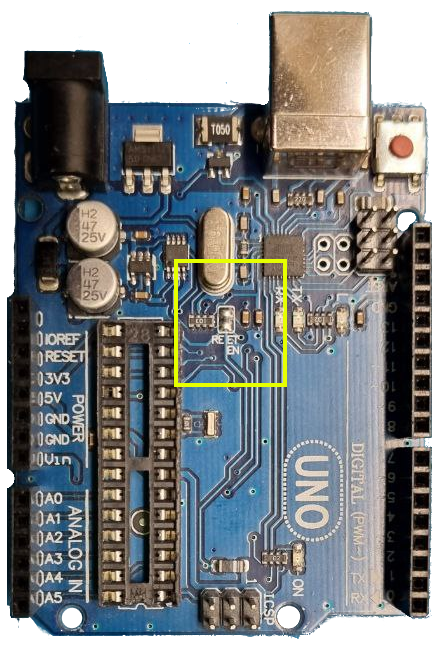
\includegraphics[width=.9\textwidth]{cap_begin.png}}
    \end{minipage}
    \begin{minipage}{.45\textwidth}
        \subfloat[][]{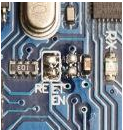
\includegraphics[width=.5\textwidth]{cap_removed.png}} \\
        \subfloat[][]{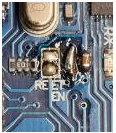
\includegraphics[width=.5\textwidth]{cap_shorted.png}}
    \end{minipage}
    \hfill
    \caption[]{Procedimento di rimozione del condensatore \texttt{C5}. Il condensatore viene rimosso (b) e successivamente la connessione viene ripistinata (c)}\label{fig:remove-c5}
\end{figure}

Tale modifica rende inoperabile il firmware presente sul controllore ATMega16U2 in quanto così facendo la linea di reset rimarrebbe asserita al livello logico 0 durante la durata della connessione con l'\texttt{host}.

Questa modifica comporta però il collegamento i componenti \texttt{RN2D} e \texttt{RN1D} i quali vanno a costituire un partitore di tensione che porrebbe la linea di reset ad un livello logico indefinito ad una tensione di 0.45V. Per questo motivo si rende necessaria una seconda modifica: è necessario isolare la resistenza \texttt{RN2D} targliando la traccia come mostrato in figura~\ref{fig:cut-rnd2}

\begin{figure}[b]
    \centering
    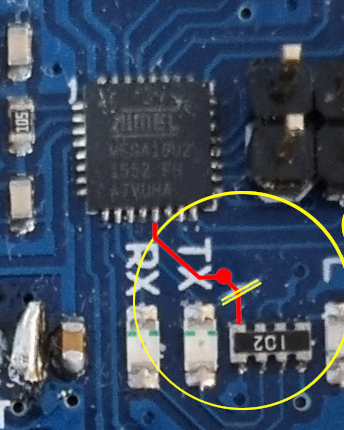
\includegraphics[width=.25\textwidth]{cut_rnd2.png}
    \caption[]{Isolamento del componente \texttt{RN2D} tagliando la traccia evidenziata.}\label{fig:cut-rnd2}
\end{figure}

Questa modifica si ripercuote negativamente sulla possibilità di eseguire il bootloader sull'ATMega16U2, in quanto è necessario che il pin 13 sia posto a 0V perchè esso possa essere caricato. Vi sono quindi tre possibilità:
\begin{enumerate}
    \item Caricare il firmware personalizzato antecedentemente alle modifiche hardware.
    \item Utilizzare un programmatore esterno tramite l'header di programmazione \texttt{ICSP1}
    \item Collegare temporaneamente durante il reset dell'ATMega16U2 la traccia tagliata con l'ausilio di uno strumento conduttivo.
\end{enumerate} 

\subsection{Riutilizzo del pulsante di reset}

La connessione per il debugging, trattasi di una linea seriale open drain, comporta che il punsante di reset presente sulla scheda non sia più funzionante, in quanto le funzionalità originali del pin di reset vengono disattivate con l'attivazione della periferica DebugWire.

La soluzione adottata consiste nell'implementazione di un soft-reset gestito dal microcontrollore ATMega16U2: La connessione del pulsante viene modificata in modo che esso sia un input letto dal firmware modificato del micro-controllore adattatore, il quale si occuperà di resettare il \textit{target} mediante l'invio di una sequenza di comandi descritta dall'algoritmo seguente:
\begin{enumerate}
    \item Halt del target (BREAK)
    \item Reset del controllore (0x07)
    \item Ripresa dell'esecuzione (0x30)
\end{enumerate}

A tal fine è necessario installare una connessione ausiliaria tramite un filo e tagliare la traccia di connessione del pulsante come mostrato dalla figura~\ref{fig:rst-rewire}

\begin{figure}[h]
    \centering
    \subfloat[][]{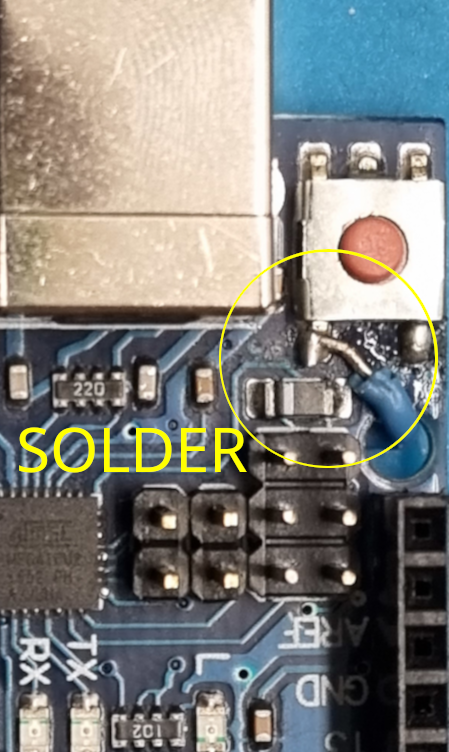
\includegraphics[width=.2\textwidth]{rst-solder-front.png}}
    \hspace{8mm}
    \subfloat[][]{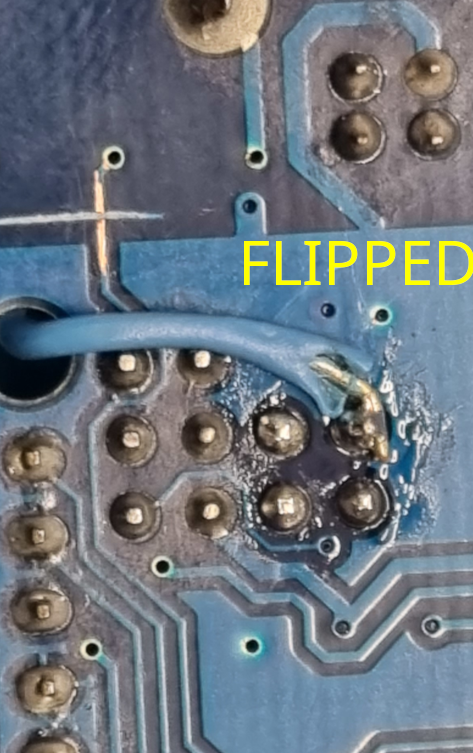
\includegraphics[width=.2\textwidth]{rst-solder-rear.png}}

    \caption[]{Procedimento di isolamento e riutilizzo del pulsante di reset mostrato dal lato superiore (a) e inferiore (b). Si noti la traccia tagliata nell'immagine (b)}\label{fig:rst-rewire}
\end{figure}


    \chapter{Implementazione}

%todo intro?


\section{Modifiche hardware alla scheda}\label{s:dw-board-mod}

Come discusso nell'introduzione la scheda \textit{Arduino UNO R3} non presenta alcun supporto al debugging o ad estensioni per tale funzione.

Questo comporta la necessità di sviluppare una nuova scheda derivata dall'architettura di \textit{Arduino UNO} --- il cui sviluppo comporterebbe un dispendio di energie e tempo non indifferenti e alte possibilità di errore --- oppure la modifica hardware e firmware di un esemplare della stessa.

Affinché sia possibile utilizzare l'interfaccia di debugging DebugWire è necessaria una connessione con pull-up diretta con il pin i reset dell'integrato.

Come è possibile osservare dall'allegato~\ref{app:r3-schematic}, L'integrato \texttt{U3} è connesso al pin di reset del target (\texttt{U4}) tramite il condensatore \texttt{C5} (si veda la figura~\ref{fig:r3-schematic-rst-detail}). Sarà dunque necessario rimuovere tale condensatore e ripristinare una connessione diretta tra i micro-controllori come evidenziato dalla figura~\ref{fig:remove-c5}.

\begin{figure}[t]
    \hfill
    \begin{minipage}{.45\textwidth}
        \subfloat[][]{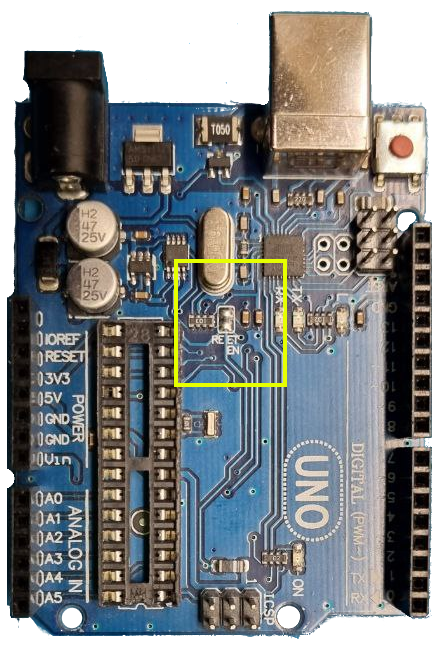
\includegraphics[width=.9\textwidth]{cap_begin.png}}
    \end{minipage}
    \begin{minipage}{.45\textwidth}
        \subfloat[][]{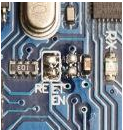
\includegraphics[width=.5\textwidth]{cap_removed.png}} \\
        \subfloat[][]{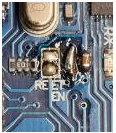
\includegraphics[width=.5\textwidth]{cap_shorted.png}}
    \end{minipage}
    \hfill
    \caption[]{Procedimento di rimozione del condensatore \texttt{C5}. Il condensatore viene rimosso (b) e successivamente la connessione viene ripristinata (c)}\label{fig:remove-c5}
\end{figure}

Tale modifica rende inoperabile il firmware presente sul controllore ATMega16U2 in quanto così facendo la linea di reset rimarrebbe asserita al livello logico 0 durante la durata della connessione con l'\texttt{host}.

Questa modifica comporta però il collegamento i componenti \texttt{RN2D} e \texttt{RN1D} i quali vanno a costituire un partitore di tensione che porrebbe la linea di reset ad un livello logico indefinito ad una tensione di 0.45V. Per questo motivo si rende necessaria una seconda modifica: è necessario isolare la resistenza \texttt{RN2D} tagliando la traccia come mostrato in figura~\ref{fig:cut-rnd2}

\begin{figure}[b]
    \centering
    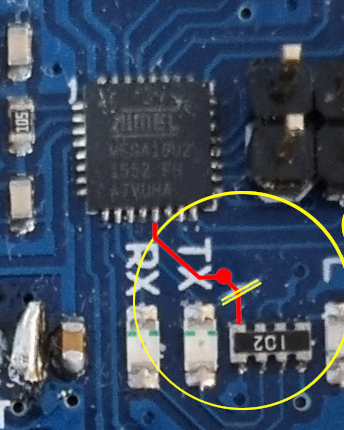
\includegraphics[width=.25\textwidth]{cut_rnd2.png}
    \caption[]{Isolamento del componente \texttt{RN2D} tagliando la traccia evidenziata.}\label{fig:cut-rnd2}
\end{figure}

Questa modifica si ripercuote negativamente sulla possibilità di eseguire il bootloader sull'ATMega16U2, in quanto è necessario che il pin 13 sia posto a 0V perchè esso possa essere caricato. Vi sono quindi tre possibilità:
\begin{enumerate}
    \item Caricare il firmware personalizzato antecedentemente alle modifiche hardware.
    \item Utilizzare un programmatore esterno tramite l'header di programmazione \texttt{ICSP1}
    \item Collegare temporaneamente durante il reset dell'ATMega16U2 la traccia tagliata con l'ausilio di uno strumento conduttivo.
\end{enumerate} 

\subsection{Riutilizzo del pulsante di reset}

La connessione per il debugging, trattasi di una linea seriale open drain, comporta che il punsante di reset presente sulla scheda non sia più funzionante, in quanto le funzionalità originali del pin di reset vengono disattivate con l'attivazione della periferica DebugWire.

La soluzione adottata consiste nell'implementazione di un soft-reset gestito dal microcontrollore ATMega16U2: La connessione del pulsante viene modificata in modo che esso sia un input letto dal firmware modificato del micro-controllore adattatore, il quale si occuperà di resettare il \textit{target} mediante l'invio di una sequenza di comandi descritta dall'algoritmo seguente:
\begin{enumerate}
    \item Halt del target (BREAK)
    \item Reset del controllore (0x07)
    \item Ripresa dell'esecuzione (0x30)
\end{enumerate}

A tal fine è necessario installare una connessione ausiliaria tramite un filo e tagliare la traccia di connessione del pulsante come mostrato dalla figura~\ref{fig:rst-rewire}

\begin{figure}[h]
    \centering
    \subfloat[][]{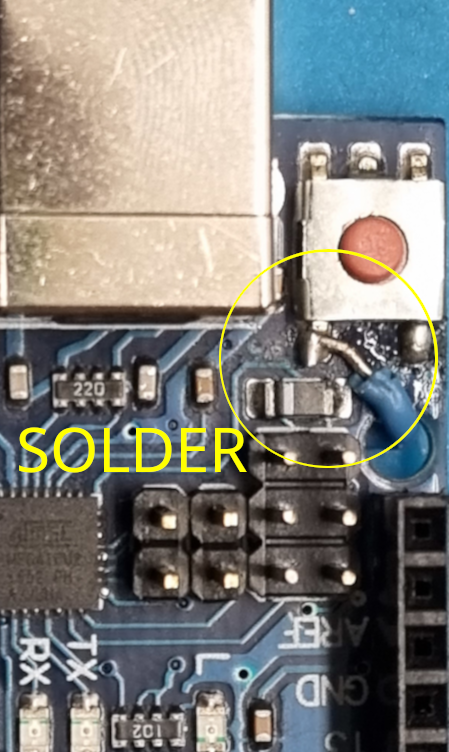
\includegraphics[width=.2\textwidth]{rst-solder-front.png}}
    \hspace{8mm}
    \subfloat[][]{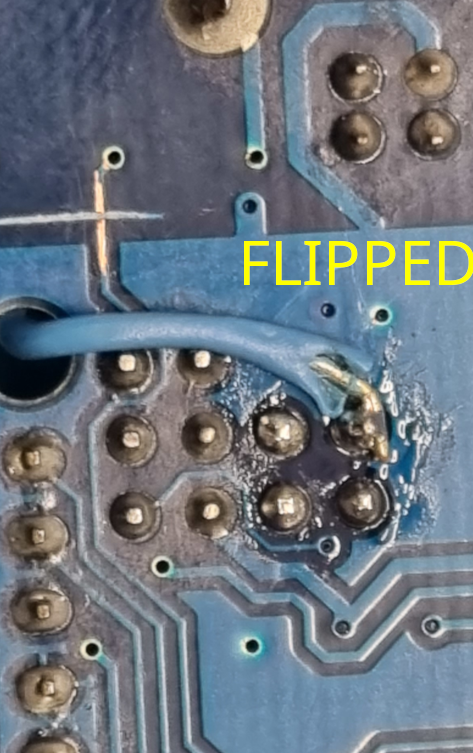
\includegraphics[width=.2\textwidth]{rst-solder-rear.png}}

    \caption[]{Procedimento di isolamento e riutilizzo del pulsante di reset mostrato dal lato superiore (a) e inferiore (b). Si noti la traccia tagliata nell'immagine (b)}\label{fig:rst-rewire}
\end{figure}

\section{Livello Fisico}

Come riportato nella sezione~\ref{ss:dw-phy}, l'interfaccia tra debug server, l'ATMega16U2, e il controllore target è costituita da una linea seriale open drain.

Si rende necessario quindi implementare tale interfaccia in modo efficiente al fine di permettere al server GDB di interfacciarsi con il \textit{target} tramite DebugWire

L'implementazione inizialmente progettata in fase di ideazione, ancora prima che fosse stabilita la piattaforma hardware, sfruttava la periferica UART presente sul controllore ATMega16U2\cite[chap. 18]{avr:m16u2}.

Al fine di implementare l'accesso alla linea open drain si rende necessario l'utilizzo di un componente aggiuntivo come mostrato nella figura~\ref{fig:od-impl}, la quale mostra due alternative di implementazione utilizzando un diodo o un transistor. 

\begin{figure}[t]
    \centering

    \subfloat[][]{
        \begin{circuitikz}
            \draw (0, 0) node[label={[font=\footnotesize]above:rxd}] {} to[short, *-] (2, 0) to[short, -] (2, 1) to[R={\(R_{pullup}\)}] (2, 2) to [short, -] (2, 2.5) to [short, -] (2.5, 2.5) to [short, -] (2.5, 3);
            \draw (2.5, 2.5) to[short, -] (3, 2.5) to[short, -] (3, 2) to[R={\(R1\)}] (3, 1);
            \draw (3,-1) node [npn,xscale=-1,anchor=B] (npn) {\reflectbox{\(Q1\)}} (npn.collector);
            \draw (3, 1) to[short, -] (3, -1);
            \draw (2, 0) to[short, *-*] (4, 0) node[label={[font=\footnotesize]above:target}] {};
            \draw (0, -2) node[label={[font=\footnotesize]above:txd}] {} to[short, *-]  (2.16, -2) to[short, -] (2.16, -1.75);
            \draw (2.16, 0) to[short, *-] (2.16, -0.5);
            \draw (2, 3) -- node[anchor=south,align=center] {VCC} (3, 3);
        \end{circuitikz}
    }
    \subfloat[][]{
        \begin{circuitikz}
            \draw (0, 0) node[label={[font=\footnotesize]above:rxd}] {} to[short, *-] (2, 0) to[short, -] (2, 1) to[R={\(R_{pullup}\)}] (2, 2) to [short, -] (2, 3);
            \draw (1.5, 3) -- node[anchor=south,align=center] {VCC} (2.5, 3);
            \draw (2, 0) to[short, *-*] (4, 0) node[label={[font=\footnotesize]above:target}] {};
            \draw (2, 0) to[short, -] (2, -0.5) to[D={\(D1\)}] (2, -1.5) to[short, -] (2, -2)  to [short, -*] (0, -2) node[label={[font=\footnotesize]above:txd}] {};
        \end{circuitikz}
    }
    \caption[]{L'immagine mostra due possibili circuiti per l'adattamento della periferica UART dell'ATMega16U2 alla linea seriale open drain.}\label{fig:od-impl}
\end{figure}

Il principio di funzionamento dei circuiti in figura~\ref{fig:od-impl} è pressoché identico: Il valore del pin txd viene replicato sulla linea di connessione con un livello logico 0 ``forte'' e un livello logico 0 ``debole'' dato dalla resistenza \(R_{pullup}\) e in entrambi i casi il pin txd viene utilizzato come collettore di corrente.
La differenza consiste nella quantità di componenti aggiuntivi e nelle prestazioni.

Il circuito (a) permette, tramite il pin \textit{txd}, di porre la differenza di potenziale \(V_{be}\) tra base ed emettitore del transistor a circa 5V --- ignorando la caduta di tensione irrilevante sulla resistenza R1 --- permettendo una corrente di base sufficiente a mandare il transistor in saturazione. Questo manda il transistor in conduzione, ed essendo in saturazione, porta la differenza di potenziale \(V_{ce}\) a circa 0.2V imponendo così la tensione sulla connessione verso il target.

Contrariamente il circuito (b) sfrutta il diodo D1 per ottenere lo stesso risultato. La differenza consta nel fatto che nel circuito (a) il transistor permette di avere una caduta di tensione minore essendo in saturazione, cosa che avviene quando il segnale \textit{txd} è zero.

I circuiti sopra mostrati sono verificati dalle simulazioni i cui risultati sono mostrati in figura~\ref{graph:sim}. In aggiunta a quanto esibito, il circuito (b) è stato simulato con un diodo schottky 1N5817 con capacitanza di 125pF per valutarne il comportamento.

\begin{figure}
    \centering
        \begin{tikzpicture}
            \begin{axis}[
                width=0.8\textwidth,
                xlabel={Tempo (S)},
                ylabel={Tensione (V)}
                ]
                \addplot table [x=t, y=v(tgt), col sep=comma, mark=none] {sims/phy-sim-bjt.csv};
                \addplot table [x=t, y=v(txd), col sep=comma, mark=none] {sims/phy-sim-bjt.csv};
                \legend{$tgt$,$txd$}
            \end{axis}
        \end{tikzpicture}\\
        \vfill
        \begin{tikzpicture}
            \begin{axis}[
                width=0.8\textwidth,
                xlabel={Tempo (S)},
                ylabel={Tensione (V)}
                ]
                \addplot table [x=t, y=v(tgt), col sep=comma, mark=none] {sims/phy-sim-diode.csv};
                \addplot table [x=t, y=v(txd), col sep=comma, mark=none] {sims/phy-sim-diode.csv};
                \addplot table [x=Time, y=V(NODE1), col sep=comma, mark=none] {sims/phy-sim-schottky.csv};
                \legend{$tgt (pn)$,$txd$}
            \end{axis}
        \end{tikzpicture}
    \caption[]{Risultati della simulazione dei circuiti in figura~\ref{fig:od-impl} con tempo di bit pari a 8\(\mu\)S}\label{graph:sim}
\end{figure}

Come è possibile notare nel secondo caso la tensione della linea \textit{tgt} non è mai inferiore a 0.7V per la giunzione \textit{pn} mentre nel caso della giunzione metallo-semiconduttore la tensione associata al livello logico 0 è pari a circa 0.15V. Bisogna però sottolineare come nel caso di un diodo schottky l'alta capacitanza causa una lentezza di commutazione non indifferente, essendo che il segnale non raggiunge mai i 5V. 


Sfruttando la periferica UART dell'ATMega16U2 risulta quindi notevolmente semplificata l'implementazione della comunicazione DebugWire, oltre a rendere possibile un approccio ad interrupt per la scrittura del firmware.

\subsection{Implementazione effettiva}

Data la scelta di riutilizzare modificando la scheda \textit{Arduino UNO R3}, si è reso necessario l'utilizzo di un solo pin (pin 13) in quanto già collegato al pin di reset dopo le modifiche apportate descritte dalla sezione~\ref{s:dw-board-mod}.

Di conseguenza si è reso necessario scrivere un'implementazione software del protocollo seriale tramite un solo pin.

La prima difficoltà di impleentazione riguarda la gestione del pin per l'utilizzo OpenDrain: la piattaforma AVR non supporta nativamente in hardware tale funzione, rendendo necessaria la gestione dello stato del pin a livello software.

Vi sono tre registri di gesione di un pin nell'architettura AVR:\ \texttt{PORTx, DDRx e PINx}. A ogni bit di questi registri è associato un pin fisico e il relativo stato.

Attraverso quanto è rappresentato nella figura~\ref{fig:avr-pin} possiamo valutare le varie condizioni nelle quali il pin fisico può trovarsi in funzione dello stato dei bit relativi ai tre registri elencati in precedenza.

\begin{figure}[t]
    \centering
    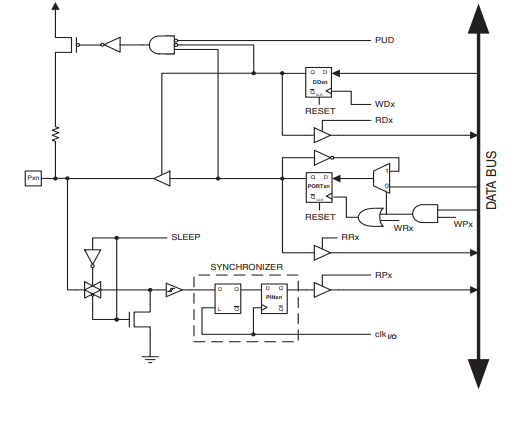
\includegraphics[width=.85\textwidth]{avr-pin-diag.png}
    \caption[Immagine ottenuta dal documento\cite{avr:m16u2}, fig. 12-2]{Diagramma funzionale dell'hardware relativo a un generico pin della famiglia AVR\cite[fig. 12-2]{avr:m16u2}}\label{fig:avr-pin}
\end{figure}

Alla scrittura del registro DDRx viene asserita la linea WDx, la quale salva lo stato del bit associato al pin nel flipflop pilotato da essa. Questo stato pilota un buffer che stabilisce se il pin stesso debba essere un input o un output.

In particolare, se lo stato salvato nel primo flipflop è 1, il pin sarà pilotato con livello logico pari allo stato salvato nel secondo flipflop in modo ``forte''.

Se invece lo stato del pin viene posto come input, ossia lo stato del primo flipflop è 0, è possibile pilotare il FET che alimenta la linea di pullup del pin. Questo accade perchè il segnale che rappresenta la direzione del pin è input negato della porta AND che controlla lo stato del pullup; per questo motivo, lo stato 0 permette alla porta di avere risultato 1 se lo stato del secondo flipflop è pari a 1, in quanto tale segnale sarebbe ignorato perchè il buffer di controllo è disabilitato.

La lettura dello stato del pin può avvenire in qualunque momento tramite la lettura del registro PINx, il quale asserisce la linea RPx e riporta lo stato salvato nello stadio di sincronizzazione.

La scrittura di tale registro viene reindirizzata al controllo del multiplexer in modo da poter invertire lo stato del pin senza averlo precedentemente letto, dimezzando la quantità di operazioni necessarie all'inversione dello stato.

Risulta quindi necessario stabilire due sequenze di operazioni per portare il pin da livello logico basso ``forte'' a livello logico alto ``debole''. In particolare la transizione da livello logico alto a livello logico basso deve avvenire precedentemente alla configurazione della direzione del pin. Questo garantisce che non vi siano possibilità di conflitti potenzialmente catastrofici, considerando il fatto che il segnale che determina l'attivazione del pullup è anche responsabile dello stato del pin. Questo problema risulta evitabile utilizzando un pullup esterno.

Analogamente per la conversione da livello logico basso a livello logico alto il cambio di stato dovrà avvenire successivamente al cambio di direzione.

Così facendo si riducono le possibilità di guasto e si minimizzano i tempi di incertezza --- considerando l'assenza di un pullup esterno --- i quali si limitano al tempo intercorso tra i due cambi di configurazione: ci sarà sempre un intervallo di tempo dove lo stato del pin sarà posto a livello logico basso e il pin posto in configurazione di input, lasciando così la connessione flottante.

In questi casi, data la durata di natura molto breve della commutazione e del periodo di incertezza, la capacitanza parassita della connessione permetterà di mantenere un livello logico costante.

\subsubsection{Implementazione del protocollo di comunicazione}

L'implementazione della comunicazione seriale emulata a livello software è soggetta a vincoli relativi al tempo di esecuzione.

L'implementazione si basa sull'utilizzo del timer TIMER1, un timer a 16 bit in grado di generare interrupt di comparazione e sul rilevamento della caduta da livello logico alto a basso per identificare un bit di inizio trasmissione.

Il concetto sul quale si basa il funzionamento consiste nel mantenere il timer in esecuzione ed eventualmente resettarne il conteggio nel caso si renda necessario una re-sincronizzazione in ricezione.

Entrambe le azioni di trasmissione e ricezione vengono implementate come una macchina a stati la quale iterazione è controllata dall'interrupt di comparazione di TIMER1.

Entrambe le funzionalità sono divide in due domini di esecuzione: l'esecuzione invocata dall'utente e la macchina a stati relativa eseguita con l'interrupt. 

La funzionalità di invio è implementata tramite un meccanismo di accodamento per due processi producer/consumer: alla prima invocazione della funzione di invio il byte viene salvato nella coda e viene abilitata la macchina a stati mostrata in figura~\ref{fig:phy-state-tx} tramite il flag \texttt{\_OD\_UART\_BUSY} la quale consumerà il dato al primo interrupt di comparazione, mentre nella seconda invocazione un secondo byte verrà inserito nella coda e la funzione potrà ritornare liberamente. 

È compito della macchina a stati riconoscere che un secondo byte è stato aggiunto alla coda \texttt{OD\_UART\_TX\_FULL} e di conseguenza essa inizierà una nuova trasmissione invece che andare allo stato \texttt{IDLE}.

\begin{figure}[t]
    \centering
    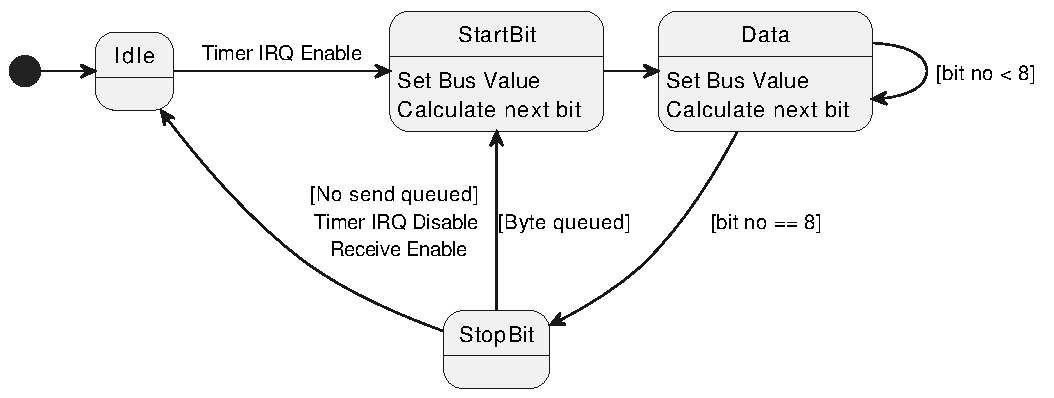
\includegraphics[width=.95\textwidth]{phy-tx-state.pdf}
    \caption[]{Macchina a stati per l'implementazione della trasmissione seriale}\label{fig:phy-state-tx}
\end{figure}

Il comportamento sopra descritto viene riassunto dalla figura~\ref{fig:phy-tx-timing}. Si noti come i cambiamenti di stato e il calcolo dei valori avvenga nell'iterazione precedente all'attuazione.
Inoltre l'immagine mostra come un eventuale aggiunta di un dato alla coda persista e venga indicata dal flag \texttt{OD\_UART\_TX\_FULL}.

Una volta terminata l'esecuzione dell'invio del dato, essendoci un ulteriore byte in coda, viene ripresa l'esecuzione immediatamente.

\begin{figure}[p]
    \checkoddpage%
    \ifoddpage%
        \begin{adjustbox}{addcode={\begin{minipage}{\width}}{\caption[]{%
            Diagramma delle tempistiche di esecuzione dell'invio di dati sulla linea seriale implementata via software.}\label{fig:phy-tx-timing}\end{minipage}},rotate=90,center}
            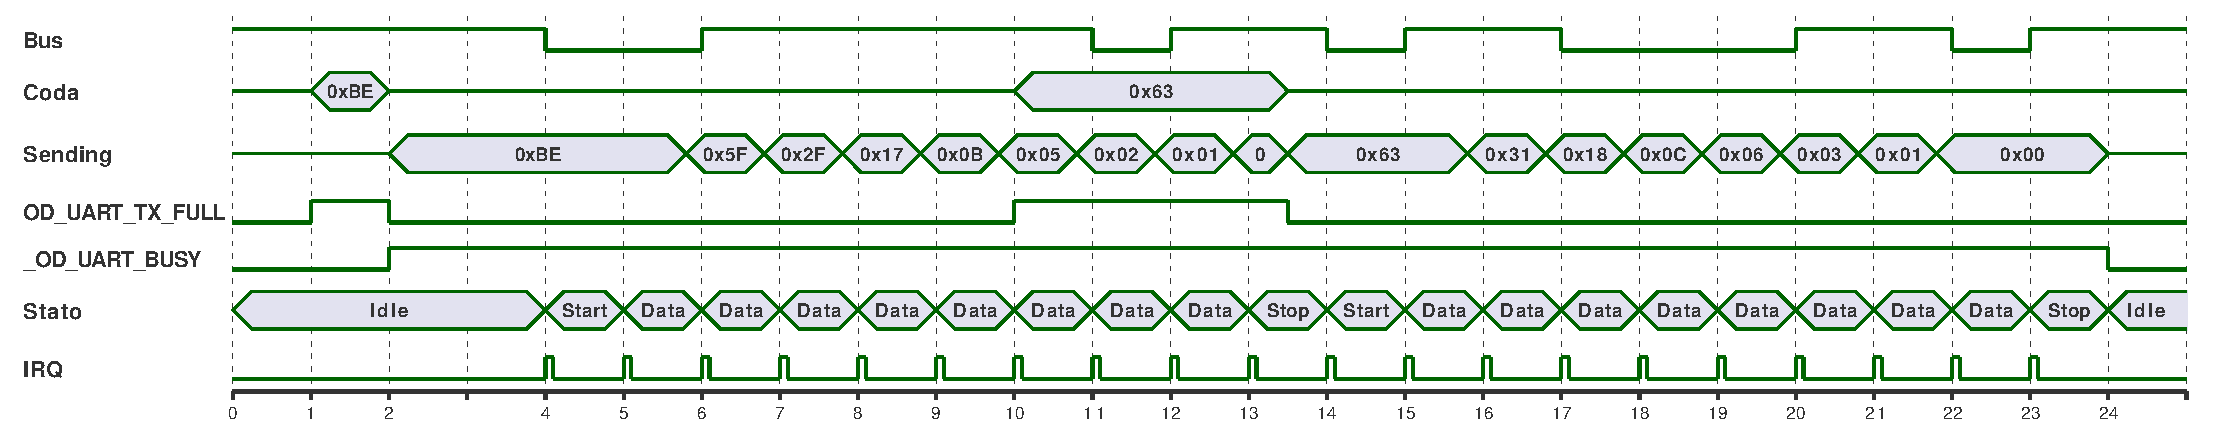
\includegraphics[width=\textheight]{phy-tx-timing.pdf}%
        \end{adjustbox}
    \else
        \begin{adjustbox}{addcode={\begin{minipage}{\width}}{\caption[]{%
            Diagramma delle tempistiche di esecuzione dell'invio di dati sulla linea seriale implementata via software.}\label{fig:phy-tx-timing}\end{minipage}},rotate=-90,center}
            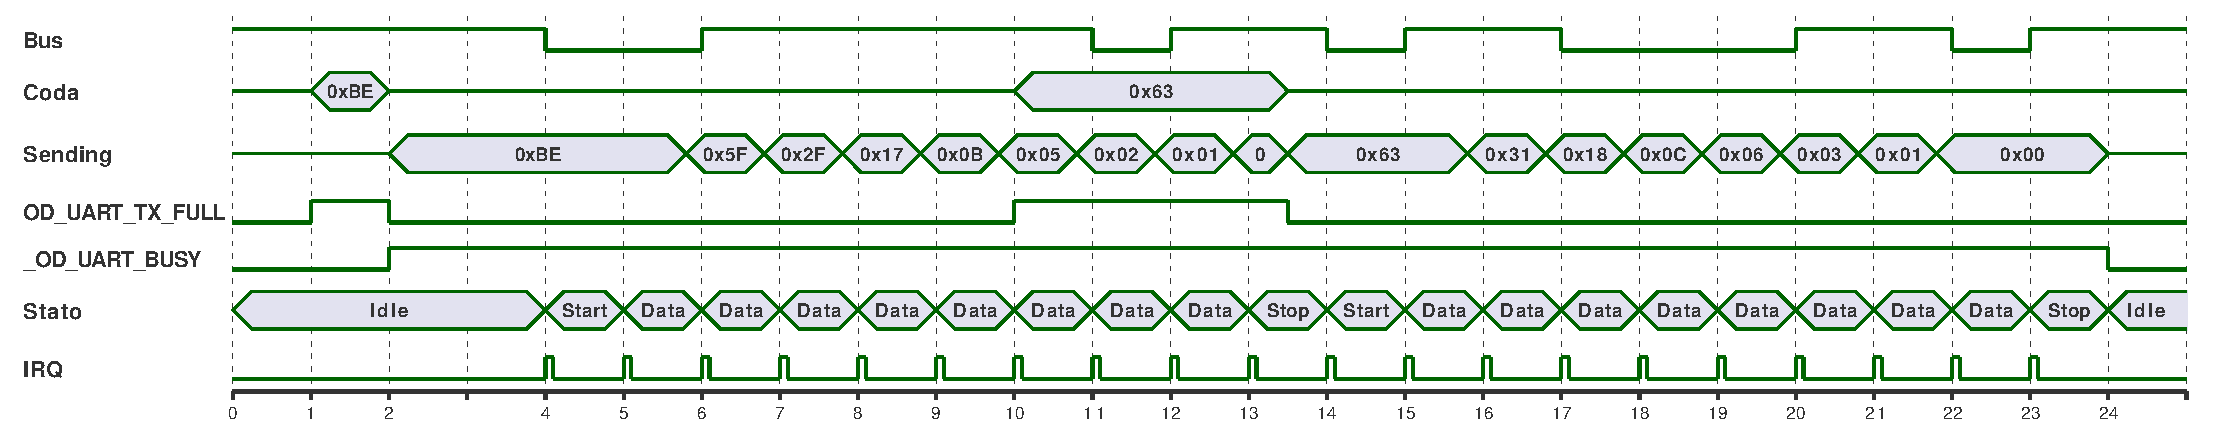
\includegraphics[width=\textheight]{phy-tx-timing.pdf}%
        \end{adjustbox}
    \fi
\end{figure}



La parte di ricezione viene implementata con una seconda macchina a stati mostrata in figura~\ref{fig:phy-rx-state} ma il primo passaggio di stato, da Idle a StartBit avviene alla ricezione di un interrupt relativo al cambiamento di stato del bus.

La ragione per cui questo passaggio debba avvenire all'avvenimento di un interrupt consiste nel fatto che il \textit{target} può inviare una risposta in qualsiasi istante temporale.

Risulta quindi necessario l'utilizzo di una struttura FIFO per il salvataggio dei dati ricevuti dalla quale poi l'utente potrà attingere durante l'esecuzione del software. In particolare il flag \texttt{\_OD\_UART\_AVAIL} indicherà la presenza di dati non ancora letti nel buffer.

Si rende quindi necessario poter ripristinare il conteggio del TIMER1 al fine di re-sincronizzare il clock di campionamento del bus al centro del bit per i motivi descritti nella sezione~\ref{ss:uart}, in particolare facendo riferimento all'equazione~\ref{eq:uart-period-receive-delay}. Questo comportamento è riassunto dalla figura~\ref{fig:phy-rx-timing}.

Alla ricezione dell'interrupt di cambio di stato la macchina a stati viene inizializzata e il timer resettato in modo che il successivo interrupt di comparazione avvenga a metà del bit successivo. Ad ogni interrupt il valore del bus viene aggiunto secondo l'equazione~\ref{eq:rx-push} al valore temporaneo fino al raggiungimento delle otto iterazioni. A questo punto lo stato passa a \texttt{StopBit}, dove il valore temporaneo viene inserito nella coda e viene asserito il flag \texttt{\_OD\_UART\_AVAIL}.

\begin{equation}\label{eq:rx-push}
    tmp_{i+1} = (bus << 7) | (tmp_i >> 1)
\end{equation}

\begin{figure}[p]
    \centering
    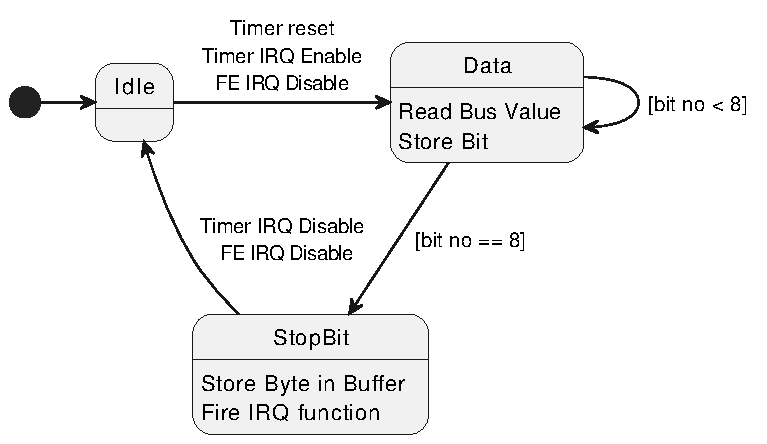
\includegraphics[width=.75\textwidth]{phy-rx-state.pdf}
    \caption[]{Macchina a stati relativa alla ricezione della seriale implementata in software.}\label{fig:phy-rx-state}
\end{figure}

\begin{figure}[p]
    \centering
    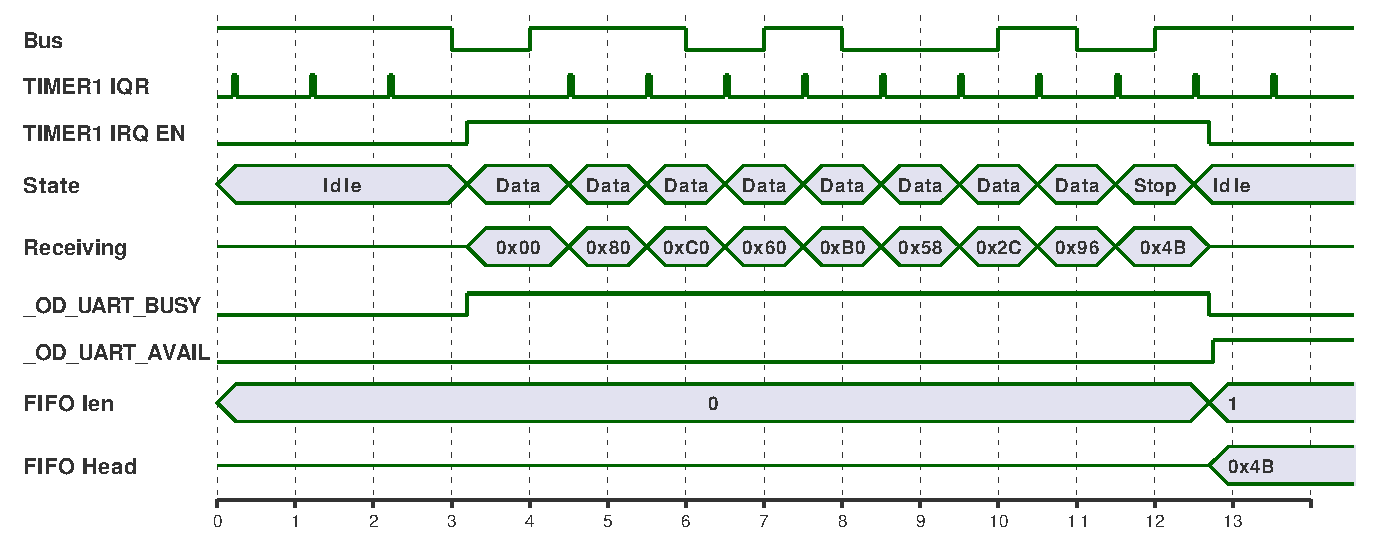
\includegraphics[width=.99\textwidth]{phy-rx-timing.pdf}
    \caption[]{Macchina a stati relativa alla ricezione della seriale implementata in software.}\label{fig:phy-rx-timing}
\end{figure}

Il listato~\ref{lst:fe-irq-management} mostra il frammento di codice per la gestione dell'inizio ricezione. 

\noindent\begin{minipage}{\textwidth}
    \begin{lstlisting}[style=C, caption={IRQ di gestione inizio trasmissione}, label=lst:fe-irq-management]
__attribute__((optimize("-Ofast"))) ISR(INT7_vect){
    cli();
    FE_IRQ_DISABLE(); //start a new rx. clear irq
    fast_flags = 0;
    uart_flags |= OD_UART_FLAG_BUSY_MASK; //set busy flag, reset flags
    TCNT1 = 0; //set counter to start at next bit. make correction for timer startup and bad things.
    TIMER_IRQ_ENABLE(); //enable timer and clear irq
    TIMER_IRQ_CLEAR();
    sei();
}
    \end{lstlisting}
\end{minipage}

È possibile osservare come nella compilazione dell'handler dell'interrupt venga privilegiata la velocità di esecuzione anziché lo spazio occupato dal compilato, e come il TIMER1 venga impostato a 0. Così facendo il campionamento avverrà verso l'inizio del bit inviato anziché alla metà del tempo di bit. 

Questo non è da considerarsi un problema data la bassa frequenza dell'insieme.

È inoltre necessario impostare \texttt{TCNT1 = OCR1A >\textcompwordmark> 2} nel caso si voglia utilizzare frequenze vicine a 125000 bit per secondo in quanto vanno considerati i tempi di esecuzione del codice e di reazione del timer. Questo valore è stato trovato sperimentalmente mediante l'uso di un analizzatore logico.

\section{DebugWire}

Grazie alla possibilità di eseguire istruzioni arbitrarie tramite l'interfaccia di debug, è possibile creare delle funzionalità non previste dal protocollo stesso ma di notevole importanza per la gestione del debug.

\subsection{Riconoscimento del target}

Durante l'inizializzazione il debugger leggerà il registro SIGNATURE DebugWire per identificare il componente.

Una sezione di memoria flash è stata dedicata al salvataggio di una struttura dati contenente le informazioni necessarie al debugging di un integrato, per cui è sufficiente cercare sequenzialmente la coincidenza del valore del registro signature rispetto al campo id.

La struttura salvata contenente gli indirizzi e le dimensioni viene mostrata con il listato~\ref{lst:struct-dw-dev}

\noindent\begin{minipage}{\textwidth}
    \begin{lstlisting}[style=C, caption={Strutture utilizzate nel codice finale per il salvataggio e la ricerca dei parametri associati al target connesso}, label=lst:struct-dw-dev]
    typedef struct dw_device_definition{
        uint16_t signature;

        uint16_t sram_base;         //first sram address after extended io
        uint16_t sram_end;          //first sram address after extended io

        uint8_t flash_page_end;     //words per page
        uint16_t flash_end;         //last flash valid word

        uint16_t eeprom_end;        //first eeporom address after io and extended io

        uint8_t reg_spmcsr;
        uint8_t reg_dwdr;
        uint8_t reg_eearl;
        uint8_t reg_eecr;
        uint8_t reg_eedr;
    } __attribute__((packed)) dw_device_definition_t;

    struct dw_devices{
        uint16_t items;
        dw_device_definition_t devices[];
    } __attribute__((packed));
    \end{lstlisting}
\end{minipage}

\subsection{Programmazione delle memorie non volatili}

In particolare il protocollo DebugWire non permette di accedere in scrittura alle memorie non volatili, impedendone così la programmazione tramite tale interfaccia.

Prendendo spunto da quanto riportato sul datasheet della maggior parte dei dispositivi AVR\cite[34]{avr:m328p}\cite[sec 26.2.5]{avr:m328p}, è possibile ideare una breve routine eseguibile passo-passo dal debugger per la scrittura di tali memorie.

Bisogna però trovare un modo per inviare il dato, o i dati, da scrivere nella memoria.

Una possibile soluzione potrebbe essere quella di scrivere il byte o la pagina in RAM e utilizzare così istruzioni \texttt{ld}, ma questo approccio richiederebbe troppe istruzioni e causerebbe lunghi tempi di programmazione.

La soluzione adottata è quella di leggere o scrivere il registro \texttt{DWDR}. Dati i test eseguiti, una scrittura del registro tramite i comandi sopra descritti (il registro si trova ad un indirizzo noto) richiede un ulteriore byte inviato sulla linea seriale che verrà salvato in tale registro\cite{site:dw-reverse-engeneering}. Analogamente la sua lettura comporta un ulteriore byte inviato dal target rappresentate il valore salvato\cite{site:dw-reverse-engeneering}.

Sono stati elaborati due frammenti di codice eseguibili dal debugger per la programmazione delle memorie non volati. Essi sono consultabili nell'appendice come documento~\ref{app:dw-flash-prog} e documento~\ref{app:dw-eeprom-prog}.

Da tali documenti possiamo osservare come il codice sia fortemente dipendente dal debugger per la preparazione del contesto, ovvero necessita che prima dell'esecuzione siano eseguite certe istruzioni di preparazione quali salvataggio dello stato dei registri e preparazione delle costanti e indirizzi nei registri utilizzati.

Inoltre la scrittura dell'algoritmo di programmazione della memoria flash è stata fatta facendo sì che non sia necessario istanziare un buffer contenente l'intera pagina da programmare precedentemente alla chiamata, bensì è possibile scrivere il buffer temporaneo a blocchi di dimensione indefinita purché venga completato prima di procedere.

Questo permette di scrivere codice a bassissimo impatto sulla quantità di memoria SRAM utilizzata per buffer temporanei, condizione necessaria per lo sviluppo su ATMega16U2 in quanto la memoria SRAM totale disponibile non supera i 512byte\cite{avr:m16u2}.

\subsection{Salvataggio stato di esecuzione}

Come anticipato in precedenza, l'esecuzione di azioni tramite debug wire comporta la sovrascrittura di alcuni registri al fine di configurare le azioni prima dell'operando GO, come mostrato dalle figure~\ref{fig:dw-reg-rw-com}~e~\ref{fig:dw-mem-rw-com}, comportando così una modifica dello stato dei registri inattesa e imprevedibile dal firmware in esecuzione.

Il solo cambio del valore del Program Counter comporterebbe la ripresa dell'esecuzione da un punto arbitrario del codice compilato senza alcun contesto logico.

È quindi necessario creare un sistema di salvataggio temporaneo dello stato in SRAM permettendone così il ripristino al termine delle operazioni.

A tal fine è stata identificata l'interdipendenza delle operazioni DebugWire e il loro utilizzo dei registri come mostrato dalla figura~\ref{fig:dw-wrt-deps}

\begin{figure}[h]
    \centering

    \resizebox{.95\textwidth}{!}{%
        \begin{tikzpicture}
            \draw (0,0) rectangle (2, 0.5) node[pos=.5] {PC};
            \draw (2,0) rectangle (4, 0.5) node[pos=.5] {HWBP};
            \draw (4,0) rectangle (6, 0.5) node[pos=.5] {r30, r31};
            \draw (6,0) rectangle (8, 0.5) node[pos=.5] {r28, r29};
            \draw (8,0) rectangle (10, 0.5) node[pos=.5] {r0};
            \draw (10,0) rectangle (12, 0.5) node[pos=.5] {IR};
            \draw (12,0) rectangle (14, 0.5) node[pos=.5] {r26, r27};
            \draw (14,0) rectangle (16, 0.5) node[pos=.5] {r1};
            \draw (0, 2) rectangle (4, 3) node[pos=.5] {REG\_RW};
            \draw (0, 4) rectangle (6, 5) node[pos=.5] {FLASH\_R, SRAM\_RW};
            \draw (10, 4) rectangle (12.5, 5) node[pos=.5] {EXE};
            \draw (12, 7) rectangle (2, 6) node[anchor=south west] {EEPROM\_RW};
            \draw (0, 8) rectangle (16, 9) node[pos=.5] {FLASH\_W};

            \draw [-stealth](1, 2) -- (1, 0.5);
            \draw [-stealth](3, 2) -- (3, 0.5);
            \draw [-stealth](4.5, 4) -- (4.5, 0.5);
            \draw [-stealth](7.3, 6) -- (7.3, 0.5);
            \draw [-stealth](9.3, 6) -- (9.3, 0.5);
            \draw [-stealth](11, 4) -- (11, 0.5);
            \draw [-stealth](13, 8) -- (13, 0.5);
            \draw [-stealth](15, 8) -- (15, 0.5);

            \draw [-stealth](2, 4) -- (2, 3);
            \draw [-stealth](11, 6) -- (11, 5);
            \draw [-stealth](12.25, 8) -- (12.25, 5);

            \draw (6.6, 8) -- (6.6, 7);
            \draw [dashed](6.6, 7) -- (6.6, 6);
            \draw [-stealth](6.6, 6) -- (6.6, 0.5);

            \draw (8.6, 8) -- (8.6, 7);
            \draw [dashed](8.6, 7) -- (8.6, 6);
            \draw [-stealth](8.6, 6) -- (8.6, 0.5);

            \draw (1, 8) -- (1, 5);
            \draw [dashed](1, 5) -- (1, 4);
            \draw [-stealth](1, 4) -- (1, 3);

            \draw (5, 6) -- (5, 5);
            \draw [dashed](5, 5) -- (5, 4);
            \draw [-stealth](5, 4) -- (5, 0.5);

            \draw (5.5, 8) -- (5.5, 7);
            \draw [dashed](5.5, 7) -- (5.5, 6);
            \draw (5.5, 6) -- (5.5, 5);
            \draw [dashed](5.5, 5) -- (5.5, 4);
            \draw [-stealth](5.5, 4) -- (5.5, 0.5);
        \end{tikzpicture}
    }

    \caption[]{Diagramma delle dipendenze di utilizzo dei registri target per le azioni DebugWire}\label{fig:dw-wrt-deps}
\end{figure}

È possibile individuare un cammino comune di salvataggio e ripristino dei registri per tutte le operazioni. In particolare è evidente come tutte le operazioni, ad eccezione di \texttt{EXE}, dipendano da \texttt{REG\_RW}, e come le operazioni di scrittura sulle memorie non volatili dipendano da scritture sugli stessi registri di \texttt{SRAM\_RW}.

La sequenza di salvataggio e ripristino viene mostrata nella la figura~\ref{fig:dw-wrt-seq}. L'immagine mostra una pila di registri per la quale, dato un punto di ingresso comune in funzione dell'azione da eseguire, sarà necessario salvare tutti i registri visitati nella discesa della pila fino al punto di uscita definito da tale operazione. Per esempio, l'azione \texttt{EEPROM\_RW} dovrà salvare i registri \texttt{PC}, \texttt{HWBP}, \texttt{Z (r30, r31)}, \texttt{IR}, \texttt{Y(r26, r27)} e \texttt{r0}. È possibile notare come i registri elencati siano anche quelli utilizzati dal codice presente al documento in appendice~\ref{app:dw-eeprom-prog}

\begin{figure}[h]
    \centering
    %\resizebox{.95\textwidth}{!}{%
        \begin{tikzpicture}
            
            \draw [fill=yellow!50] (0,0) rectangle (3, 1) node[pos=.5] {r1};
            \draw [fill=orange!50] (0,1) rectangle (3, 2) node[pos=.5] {X};
            \draw [fill=green!50] (0,2) rectangle (3, 3) node[pos=.5] {Y, r0};
            \draw [fill=blue!50] (0,3) rectangle (3, 4) node[pos=.5] {IR};
            \draw [fill=brown!50] (0,4) rectangle (3, 5) node[pos=.5] {Z};
            \draw [fill=gray!50] (0,5) rectangle (3, 6) node[pos=.5] {PC, HWBP};

            \draw (-0.3, 0) rectangle (0, 6);
            \draw [-stealth] (-0.15, 5.5) -- (-0.15, 0.5);

            \draw [stealth-] (-0.3, 5.5) -- (-1.5, 5.5) node[left] {All actions};
            \draw [stealth-] (-0.3, 3.5) -- (-1.5, 3.5) node[left] {EXE};

            \draw [-stealth] (3, 5.5) -- (4.5, 5.5) node[right] {REG\_RW};
            \draw [-stealth] (3, 4.5) -- (4.5, 4.5) node[right] {FLASH\_R, SRAM\_RW};
            \draw [-stealth] (3, 2.5) -- (4.5, 2.5) node[right] {EEPROM\_RW};
            \draw [-stealth] (3, 1.5) -- (4.5, 1.5) node[right] {FLASH\_CLEAR\_PAGE};
            \draw [-stealth] (3, 0.5) -- (4.5, 0.5) node[right] {FLASH\_W};
            \draw [-stealth] (3, 3.5) -- (4.5, 3.5) node[right] {EXE};
        \end{tikzpicture}
    %}

    \caption[]{Diagramma dei salvataggi e ripristini dei registri in funzione dell'operazione da eseguire}\label{fig:dw-wrt-seq}
\end{figure}

\subsection{Software Breakpoints}

L'aggiunta della possibilità di scrivere la memoria flash consente l'implementazione dei software breakpoints.

Un breakpoint è un indicatore associato a un indirizzo di memoria dove il codice è in esecuzione con il fine di interrompere l'esecuzione dell'algoritmo e passare il controllo al debugger per effettuare le operazioni di analisi e ispezione.

Questi consistono nella sovrascrittura di un'istruzione con l'opcode corrispondente a \texttt{BREAK} causando così l'halt della cpu e l'intervento del debugger prima dell'esecuzione della stessa.
Alla ripresa dell'esecuzione il debugger caricherà in memoria l'istruzione originale e riprenderà il flusso del codice.

Un primo approccio per la scrittura del codice relativo a questa feature consiste nell'aggiornare la memoria flash scrivendo un'istruzione BREAK\footnote{0x0000} non appena possibile e salvare in una struttura dati la coppia \[<indirizzo>:<opcode>\]

Un possibile algoritmo viene esibito di seguito. Questo algoritmo ha un impatto sull'utilizzo della memoria SRAM di 18 byte facendo uso del fatto che è possibile riempire il buffer di scrittura prima della cancellazione della pagina.

Sia \(address\) l'indirizzo dell'istruzione da sostituire (word address), \(pagelen\) il numero di word in una pagina.

\begin{enumerate}
    \item Salvataggio dei registri come definito in figura~\ref{fig:dw-wrt-seq} per l'azione \texttt{FLASH\_W} (14 byte)
    \item Poniamo l'indirizzo di pagina, utilizzando 2 byte, come \[pageaddr = \left\lfloor\frac{address}{pagelen}\right\rfloor pagelen\] 
    \item Iniziamo la scrittura di una pagina e, per ogni indirizzo da \(pageaddr\) a \(address\) (escluso), leggiamo in una variabile temporanea (2 byte) il valore della memoria flash a quell'indirizzo e aggiungiamo al buffer di scrittura presente nell'integrato.
    \item Scriviamo del buffer l'istruzione BREAK.\@ 
    \item Per ogni indirizzo da \(address + 1\) a \(pageaddr + pagelen - 1\) popoliamo il buffer con quanto letto. 
    \item Eseguiamo l'azione Page Clear all'indirizzo \(pageaddr\)
    \item Eseguiamo l'azione di programmazione della pagina.
    \item Ripristiniamo lo stato dei registri invertendo quanto eseguito al punto 1.
\end{enumerate}

Quanto riportato, seppur una soluzione valida, causa un deterioramento della memoria flash e innalza notevolmente i tempi di debug, inserendo attese notevoli tra il posizionamento di un breakpoint e un altro.

L'algoritmo finale risolve queste problematiche adottando una gestione ``\textit{lazy}'' dei breakpoint e accorpando modifiche alle pagine di memoria flash solo al momento precedente all'esecuzione.
Questo permette di evitare tutte le riscritture date dall'eventuale indecisione del programmatore o errori di puntamento.

Un breakpoint software viene definito con la struttura presentata nel listato~\ref{lst:dw-swbp-struct}. I flag \texttt{active} e \texttt{stored} permettono di identificare le azioni da intraprendere al momento dell'applicazione delle modifiche in memoria.

\noindent\begin{minipage}{\textwidth}
    \begin{lstlisting}[style=C, caption={Struttura utilizzata per il salvataggio dei riferimenti ai breakpoint software}, label=lst:dw-swbp-struct]
    typedef struct dw_sw_brkpt{
        uint16_t address;
        uint16_t opcode;

        uint8_t active : 1;
        uint8_t stored : 1;
    } dw_sw_brkpt_t;
    \end{lstlisting}
\end{minipage}

In particolare si ha che è necessario eseguire un'azione in memoria se i due flag sono discordanti: se un breakpoint è stato abilitato ma non è stato scritto in memoria sarà necessario sostituire l'istruzione presente all'indirizzo \(address\), mentre se un breakpoint è salvato (\texttt{stored} = 1) ma disabilitato sarà necessario ripristinare \(opcode\) all'indirizzo specificato.

Nel caso di aggiunta o rimozione di un breakpoint l'indirizzo viene ricercato all'interno della lista di breakpoint precedentemente definiti comparando l'indirizzo. Se il breakpoint era stato precedentemente definito allora il riferimento viene modificato impostando la variabile \texttt{active} al valore consono. In caso contrario viene creato un nuovo riferimento in coda.

Prima della ripresa dell'esecuzione la lista di breakpoint viene ordinata mediante insertion sort secondo in seguenti criteri:
\begin{itemize}
    \item se due riferimenti sono entrambi non salvati e inattivi non viene effettuata l'inversione e sono considerati uguali ignorando l'indirizzo.
    \item se il primo riferimento è inattivo e non salvato mentre il secondo è o salvato o attivato, allora viene eseguita l'inversione
    \item se sono tutti e due attivi o salvati, vengono comparati gli indirizzi e avviene l'inversione se il primo indirizzo è maggiore del secondo.
\end{itemize}

Così facendo si ottiene una lista di riferimenti ordinati per indirizzo crescente con i riferimenti da eliminare posti in coda a scapito di quest'ultimo, permettendo quindi la rimozione dei riferimenti inattivi e non salvati perché non più esistenti partendo dal fondo e eliminando fino a trovare un riferimento attivo o salvato.

Ora risulta possibile accorpare le scritture in memoria con un algoritmo simile a quanto riportato in precedenza considerando però la presenza di più breakpoint per pagina.

Sarebbe possibile rendere la ricerca e l'ordinamento più efficiente utilizzando algoritmi quali ricerca binaria e qsort ma non è stati ritenuto necessario essendo il numero massimo di riferimenti limitato a venti.

\section{Server GDB}

\section{Real Time Terminal}

Come precedentemente anticipato, questo progetto mira a costituire un insieme di strumenti e funzionalità per il supporto del programmatore alla programmazione nel mondo embedded AVR.\@

Nei capitoli precedenti è stata discussa l'implementazione di un server GDB per effettuare il debugging sul controllore e permettere l'ispezione in loco degli effetti dei programmi e l'alterazione delle risorse durante l'esecuzione a fini diagnostici. 

Affiancata alla pratica del debugging possiamo classificare un'altro metodo diagnostico: il \textit{logging}.

Questa seconda pratica --- spesso usata in modo scorretto per analizzare un problema in una porzione di codice --- consente di generare messaggi analizzabili successivamente a fine di \textit{auditing}, ovvero l'analisi di messaggi di log passati per individuare malfunzionamenti o vulnerabilità inattesi e imprevisti.

I messaggi di log sono anche utili per individuare in quale macro area del codice si trova un possibile baco per poi indagare tramite debugger una volta identificata la causa scatenante.

La questione diviene velocemente come implementare tale funzionalità sulla piattaforma AVR.\@ La maggior parte dei progetti e delle piattaforme utilizza la periferica UART del target al fine di comunicare con l'host impedendone così l'utilizzo da parte del programmatore per comunicare con altre periferiche. Alcune piattaforme hanno ottimizzato questo utilizzo dedicando la linea seriale anche alla programmazione, riducendo però lo spazio disponibile nella memoria flash in quanto tale operazione deve essere svolta da un programmatore. 
    \chapter{Ambiente di sviluppo}

In questo capitolo saranno discusse le funzionalità e le possibilità offerte dal progetto in questione a favore del programmatore, nonché i vantaggi e le migliorie apportate nel processo di sviluppo.

La difficoltà principale che un programmatore si trova ad affrontare nell'intraprendere un percorso di apprendimento della programmazione embedded consiste nel ritrovarsi in un mondo completamente diverso di gestione del software e ambienti di sviluppo. Vi è poi l'assoluta differenza del processo di programmazione e debug da un comune applicativo per calcolatore.

Sebbene l'approccio a una nuova piattaforma hardware con differenti specifiche e funzionalità e, spesso, con un \textit{instruction set} limitato e non famigliare possa sembrare un ostacolo impegnativo, nella realtà, grazie a strumenti quali compilatori come \textit{gcc} e \textit{rustc}, è possibile scrivere notevoli porzioni di codice completamente indipendenti dall'architettura del dispositivo finale.

La difficoltà principale per lo sviluppatore nell'approcciarsi allo sviluppo di una piattaforma embedded è di fatto l'adattarsi ad un nuovo ambiente e strumenti spesso proprietari e male o per nulla documentati.

Un'ulteriore difficoltà che limita l'accesso di nuovi sviluppatori verso il mondo embedded è la necessità di strumenti proprietari e costosi per programmare e \textit{debuggare} hardware, oltre al costo fisico di schede per la prototipazione.

Questi fattori sopra elencati hanno permesso alla società \textit{Arduino~s.r.l.} di entrare nel mercato dei dispositivi embedded mirando ad un pubblico inesperto e desideroso di approcciare una nuova pratica\cite{site:arduino-about}.

L'ecosistema Arduino è la scelta adottata dalla maggior parte di hobbisti e corsi di introduzione al mondo dell'elettronica digitale, motivati dalla dimensione della \textit{community}\footnote{Supporto di altri utenti fornito per mezzo di forum e mezzi anche non gestiti dall'azienda produttrice}, dal supporto, dagli strumenti sviluppati compatibili e semplici e dalla quantità di librerie \textit{open source} disponibili.

Non vi è dubbio sulla versatilità e la facilità di apprendimento della programmazione embedded AVR tramite la piattaforma.

Date le motivazioni e l'obiettivo dell'azienda d'Ivrea, è possibile osservare come la piattaforma e gli strumenti software non siano ottimali per uno sviluppo professionale o più complesso e ottimizzato.

\begin{figure}
    \centering
    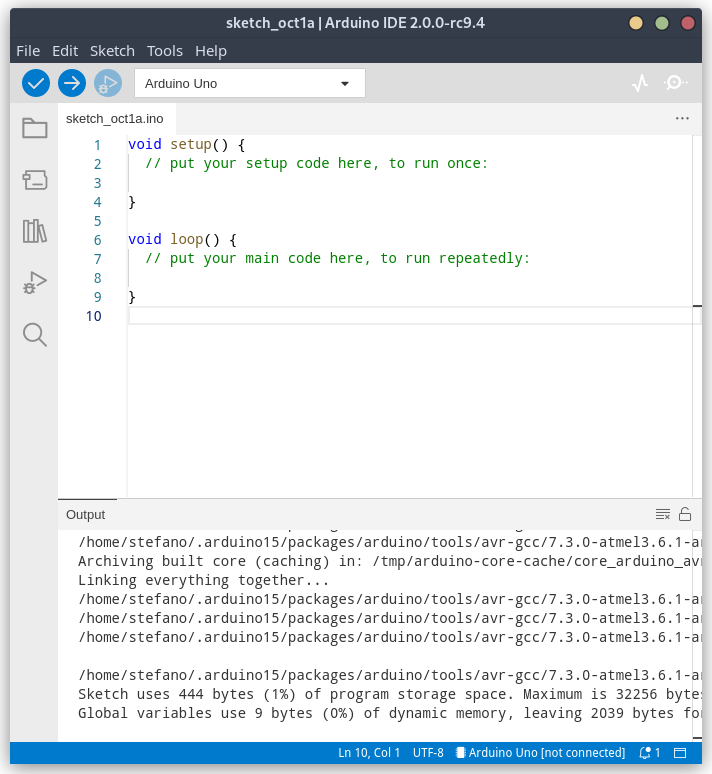
\includegraphics[width=.6\textwidth]{arduino-ide.png}
    \caption[Immagine del software Arduino IDE v2]{Finestra di programmazione dell'ambiente di sviluppo Arduino IDE v2}\label{fig:arduino-ide}
\end{figure}

Come è possibile osservare l'ambiente di sviluppo \textit{Arduino IDE} mostrato in~\cref{fig:arduino-ide} presenta un insieme notevolmente limitato di funzioni e un'interfaccia fortemente semplificata. È però possibile osservare la presenza di un indicatore di debug: questo è solo disponibile con schede ARM a 32 bit più prestazionali. La funzionalità di debug non è presente sulle schede AVR.\@

Data l'assenza del \textit{debugger} per la piattaforma AVR, gli utenti sono obbligati all'utilizzo di logging tramite connessione seriale per analizzare il flusso del codice, pratica fortemente inefficiente per motivi prestazionali e per problemi di codifica dell'informazione.

L'utilizzo del server GDB sviluppato nel corso di questo elaborato garantirebbe nuove possibilità e efficienza, risultano però complesso e poco intuitivo in quanto dotato di sola interfaccia testuale come mostrato dalla~\cref{fig:gdb-cli}

\begin{figure}
    \centering
    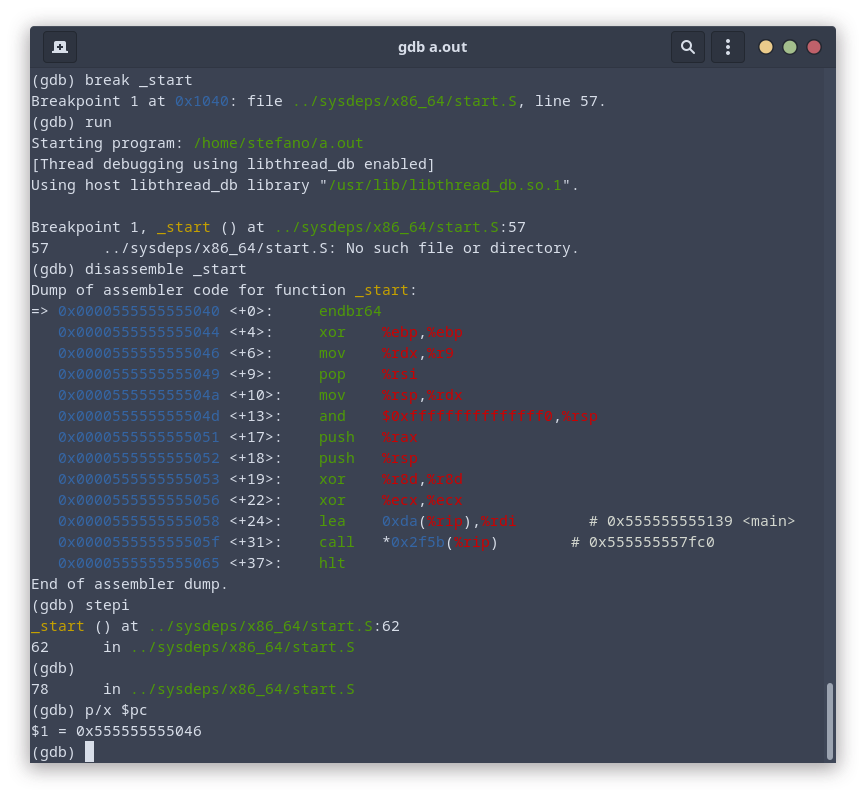
\includegraphics[width=.7\textwidth]{gdb-cli.png}
    \caption[]{Immagine di una sessione di debug da linea di comando}\label{fig:gdb-cli}
\end{figure}

Risulta quindi necessario sviluppare un insieme di strumenti che possano essere integrati nella maggior parte degli ambienti di sviluppo senza difficoltà, permettendo così di superare una delle limitazioni sopra descritte, ovvero la difficoltà di adottare un ambiente di sviluppo nuovo e mal documentato, permettendo l'utilizzo di una piattaforma nota e configurabile.

\section{CMAKE}\label{s:cmake}

Al fine di rendere la compilazione una procedura universale e generica è stato deciso l'utilizzo di un software di automazione del processo di compilazione altamente integrabile. Tale software è \textit{CMAKE}.

Esso permette di descrivere ad un livello più astratto gli obiettivi della compilazione e di impostare alcune variabili di configurazione per poi generare una procedura di compilazione in funzione delle librerie disponibili e delle caratteristiche dell'\textit{host}, semplificando la scrittura di codice interoperabile.

Inoltre, al fine di garantire interoperabilità tra ambienti di sviluppo, è stato deciso di affidare tutte le azioni di upload del codice a processi esterni che CMAKE permette di lanciare come degli obiettivi personalizzati.

L'integrazione con l'ambiente di sviluppo è invece affidata ad eventuali plugin per lo stesso o all'implementazione nativa del supporto per CMAKE.\@

Il~\cref{lst:cmake-target} mostra come un generico obiettivo di compilazione e programmazione viene descritto per poi essere tramutato in una procedura di compilazione.

È possibile notare come un singolo obiettivo per un dispositivo della piattaforma sia definito da tre distinti obiettivi concatenati e interdipendenti.

\noindent\begin{minipage}{\textwidth}
    \begin{lstlisting}[language=CMAKE, caption={Definizione di un target di compilazione e upload per un dispositivo AVR}, label=lst:cmake-target]
function(avrtarget targetName port)
    add_executable("${targetName}-elf" ${ARGN})
    target_link_options("${targetName}-elf" PUBLIC -Xlinker -T ${CMAKE_SOURCE_DIR}/cmake/linker/${MCU}.ld)
    add_custom_target(
        "${targetName}-bin" 
        COMMAND ${CMAKE_OBJCOPY} -O ihex -R .eeprom -R .fuse -R .lock -R .signature './${targetName}-elf' './${targetName}.hex';
        COMMAND ${CMAKE_OBJCOPY} -O ihex -j .eeprom './${targetName}-elf' './${targetName}.eeprom.hex';
        COMMAND ${CMAKE_SIZE} --mcu=${MCU} -C './${targetName}-elf';
        DEPENDS "${targetName}-elf"
    )
    add_custom_target(
        "${targetName}-upload"
        COMMAND python host_software/flash.py --port ${port} --flash './${targetName}.hex' --mcu ${MCU}
        USES_TERMINAL
        DEPENDS "${targetName}-bin"
    )
endfunction()

avrtarget(main main.c io.c)
target_link_libraries(main-elf rtt)
    \end{lstlisting}
\end{minipage}

In particolare sia \(main\) il nome generico assegnato all'obiettivo avr in sviluppo. La procedura di compilazione generata da CMAKE conterrà tre sotto obiettivi nominati
\begin{itemize}
    \item \textbf{main-elf}: obiettivo di compilazione effettivo dove il compilatore (\textit{avr-gcc}) verrà impiegato e genererà un file contenente codice eseguibile e informazioni di debug
    \item \textbf{main-bin}: obiettivo di utilità che estrarrà dal file \textit{build/main-elf} i file in formato \textit{ihex}\footnote{Intel Hexadecimal Format} per la programmazione delle memorie persistenti. Tali file sono una rappresentazione compressa del formato esadecimale\cite{site:ihex} e rappresentano le memorie bit per bit.
    \item \textbf{main-upload}: l'esecuzione di questo obiettivo esegue uno script che, dialogando con il server gdb, permette la scrittura della memoria flash e di conseguenza la programmazione senza uscire dalla modalità DebugWire.
\end{itemize}


\section{Ambiente di programmazione}

Per quanto riguarda l'ambiente di sviluppo, verrà commentata a seguire una configurazione di \textit{Visual Studio Code}.

La scelta di questo editor di testo è data dalla sua grande diffusione\cite{site:vscode-connect-2017} e dalla sua facilità di estensione tramite un sistema di plugin, con i quali diviene di fatto un ambiente di sviluppo integrato (IDE).

Inoltre, lo sviluppo dell'applicativo tramite la piattaforma \textit{Electron}\cite{site:vscode-about}, garantisce la compatibilità con una fetta notevolmente estesa di dispositivi oltre che alla possibilità di proporre l'applicativo tramite interfaccia web\cite{site:electron}. 

Grazie alla scelta discussa nella~\cref{s:cmake}, al fine di implementare un processo di lavoro interamente integrato nell'ambiente di sviluppo, è sufficiente configurare un plugin per il supporto al software di automazione CMAKE come mostrato dalla~\cref{fig:vscode-cmake-plugin}.\@

\begin{figure}
    \centering
    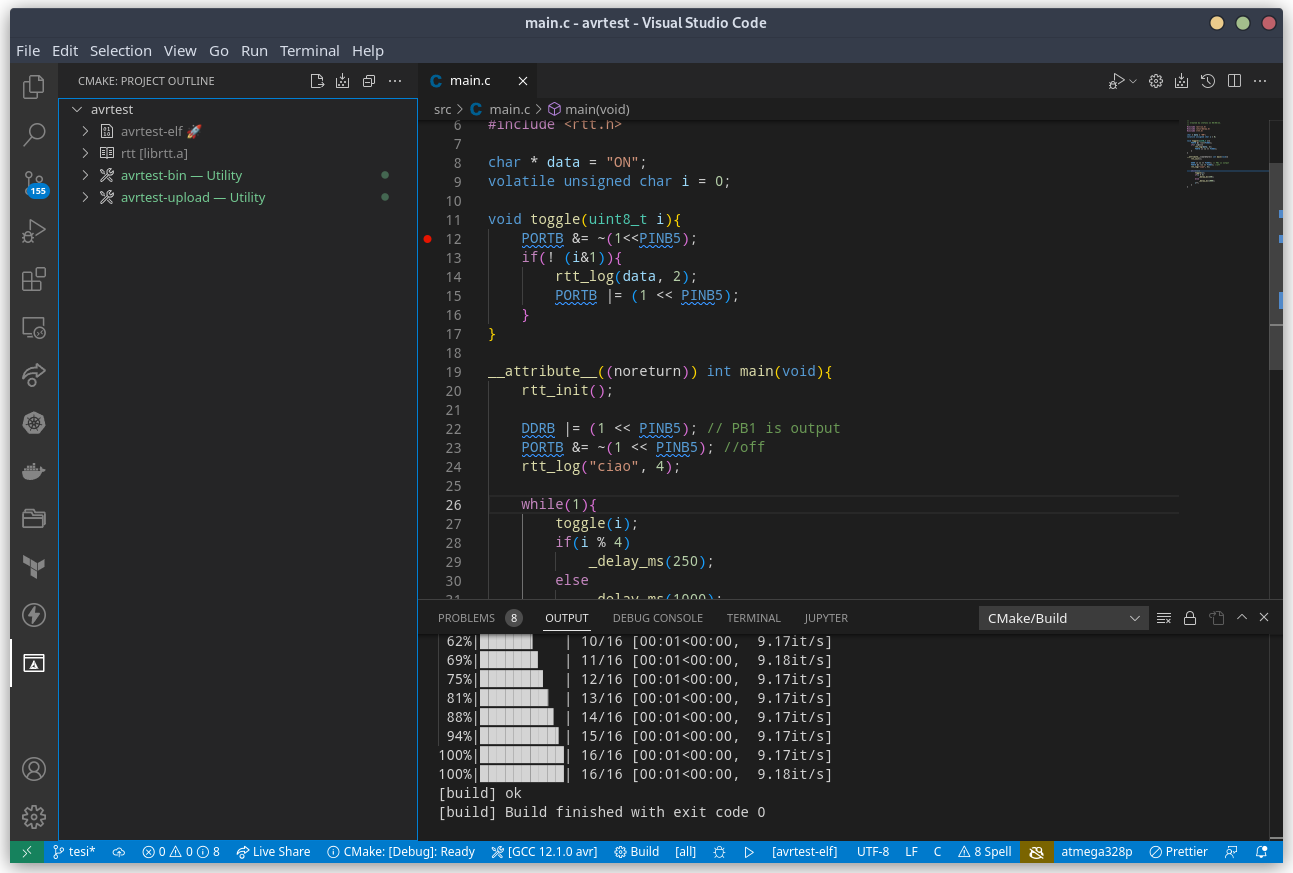
\includegraphics[width=.8\textwidth]{vscode-cmake.png}
    \caption[Immagine del software Visual Studio Code]{Visual Studio Code con il plugin CMake installato}\label{fig:vscode-cmake-plugin}
\end{figure}

Nella figura mostrata è possibile identificare la lista di obiettivi rilevati dal file di configurazione (\texttt{CMakeFile.txt}) come mostrati dalla~\cref{s:cmake}. Nel riquadro presente nella parte inferiore dell'immagine è possibile osservare l'output del comando di caricamento nella memoria flash del target del firmware compilato.

Grazie ad un'altra serie di plugin sviluppata direttamente da Microsoft è possibile implementare il supporto al linguaggio di programmazione integrando anche uno strumento di assistenza alla scrittura del codice con la possibilità di visualizzare suggerimenti inerenti a quanto viene scritto.

È anche possibile configurare l'ambiente di lavoro per l'utilizzo di un linguaggio compilato come Rust\cite{site:avrrust}, grazie all'utilizzo di librerie di astrazione dell'hardware\cite{site:arduino-hal-rust} e il supporto al compilatore avr-gcc.

In quest'ultimo caso il linguaggio e l'infrastruttura della community permette di fare affidamento su svariate librerie disponibili tramite l'utilizzo di un package-manager (\texttt{cargo}\cite{site:cargo-book})

È evidente come l'impiego di un singolo applicativo fortemente utilizzato possa offrire una vastità di scelte inimmaginabile riguardo la composizione del progetto mantenendo costantemente l'utente vicino al proprio \textit{modus operandi} con il quale abitualmente sviluppa software, garantendo elevata efficienza ed ergonomicità.

Osservando la costituzione dell'applicativo più in generale possiamo sottolineare come sia possibile configurare un processo di compilazione personalizzato pur mantenendo la compatibilità con il sistema progettato semplicemente integrando e supportando la possibilità di \textit{debuggare} il codice tramite GDB e avendo gli strumenti necessari per generare un file binario per la programmazione. 

Una volta completata la configurazione è possibile utilizzare le piene potenzialità dell'ambiente di sviluppo integrato come mostrato in~\cref{fig:vscode-debug}.

\begin{figure}
    \centering
    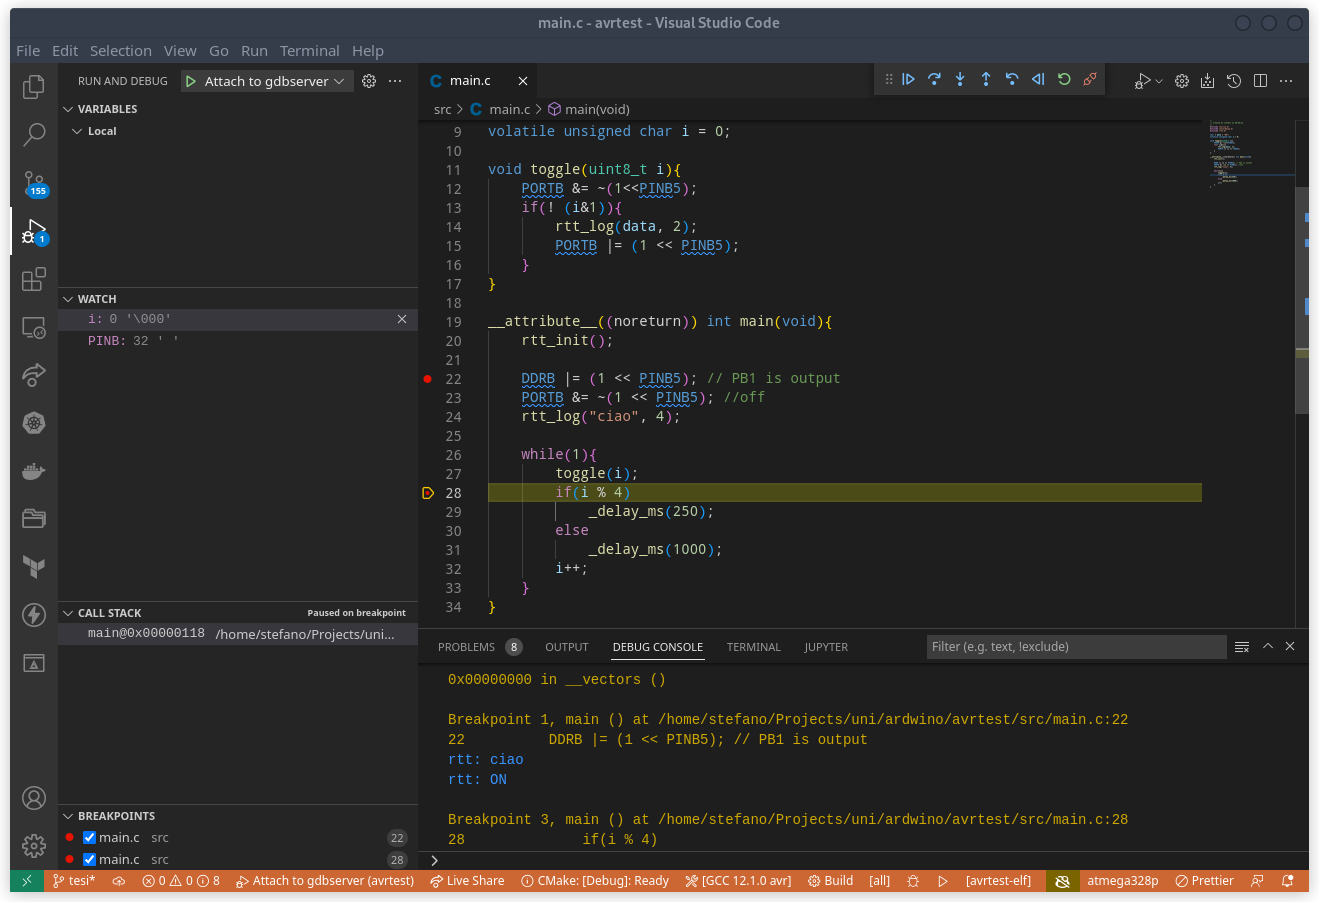
\includegraphics[width=.8\textwidth]{vscode-dbg.png}
    \caption[Immagine del software Visual Studio Code]{Visual Studio Code in modalità di debugging}\label{fig:vscode-debug}
\end{figure}

È possibile osservare come, abilitando il plugin di debug, sia disponibile un riquadro dedicato alla visualizzazione delle informazioni ottenute dal client GDB sul lato sinistro, mentre è identificabile nella parte sottostante l'output del terminale RTT (\cref{s:rtt}) evidenziato in colore blu.

Infine è osservabile la decorazione del codice durante il processo di debug come descritto dalla~\cref{ss:code-decoration}
    \chapter*{Conclusioni e Sviluppi Futuri}
\addcontentsline{toc}{chapter}{Conclusioni e Sviluppi Futuri}

Si è visto che è possibile sviluppare una serie di strumenti in grado di supportare la programmazione mediante l'introduzione di nuove funzionalità e astrazioni.

Grazie alle risorse citate e agli esperimenti eseguiti durante lo sviluppo di questi sistemi è stato possibile ideare un firmware in grado di adattare un protocollo di \textit{debugging} comunemente utilizzato a un set ridotto e non documentato di comandi verso il dispositivo target.

Lo sviluppo di tale firmware ha necessitato di continue prove e riformulazioni al fine di ottenere una versione funzionale ed efficiente. Tutt'ora la stabilità del sistema non è assoluta, in quanto esistono svariati casi e sequenze per cui è necessario effettuare un riavvio forzato del controllore, ma tali controlli e casi eccezionali non sono stati sviluppati in quanto lasciati a futuri sviluppi.

Inoltre la dimensione finale del codice compilato raggiunge i \SI{15}{KiB}, dimensione limite per la memoria di 16 KiB se si tiene conto della regione dedicata al bootloader. Il vincolo dato dalla dimensione della memoria è dato dall'adattamento all'utilizzo della scheda \textit{Arduino UNO}, la quale monta il controllore ATMega16U2 con capacità di memoria ridotta. Un possibile sviluppo futuro potrebbe consistere nel valutare il passaggio a un ATMega32U2 o ATMega32U4 per sfruttare al meglio le loro potenzialità maggiorate quali memoria flash di \SI{32}{KiB} e un totale di \SI{2.5}{KiB} di memoria SRAM\cite{avr:m16u4}.

Sarà possibile sviluppare un hardware ``\textit{Arduino Compatibile}'' --- argomento al di fuori del corso di studio --- il quale permetterebbe l'implementazione di una topologia e circuiteria che possa agevolare l'implementazione dei protocolli fisici e ridurre così le dimensioni del compilato sfruttando la periferica UART.\@
Così facendo sarebbe possibile l'implementazione di nuove funzionalità accessorie.

Ulteriori difficoltà sono state superate nello sviluppo dell'interfaccia con l'\textit{host} tramite USB.\@ Il protocollo USB è notevolmente complesso e vasto; lo sviluppo di tale parte del firmware ha necessitato di una quantità considerevole di tempo e prove al fine di comprendere al meglio le logiche utilizzate dalla libreria LUFA.\@

Infine, grazie alla versione corrente del firmware presente sull'ATMega16U2 e dalle sue funzionalità di debug, sarà possibile sviluppare una versione migliorata dello stesso sfruttando le possibilità che questo progetto offre. Si noti che il codice è stato sviluppato senza l'ausilio di strumenti di debug per quanto enunciato nell'introduzione:
\begin{center}
    \textit{Il sistema ultimato consisterà in un set di strumenti complementari e modifiche apportabili alla scheda sopra descritta in modo che chiunque sia in grado di utilizzarli e applicarli, sviluppato interamente con strumenti e dati disponibili al pubblico tramite la rete internet e senza l'uso di strumenti e hardware proprietari.}
\end{center}

Sarà dunque possibile sviluppare una nuova versione del firmware avvantaggiandosi degli strumenti di debug e log forniti da questa versione.

Al fine di poter pubblicare questa ricerca con licenza open source non sono stati utilizzati strumenti e software proprietari \textit{Microchip} o \textit{Atmel}. Questo comporta l'impossibilità di utilizzare programmatori proprietari in grado di fornire un'interfaccia di debug e di sfruttare le funzionalità di software quali \textit{Atmel Studio} in grado di utilizzare al meglio tali strumenti.

Il software, gli strumenti e le configurazioni sono state pubblicate sotto licenza \textit{Apache License 2.0}\footnote{https://www.apache.org/licenses/LICENSE-2.0}.
    
    \nocite{*}
\printbibliography[title={Bibliografia e Sitografia}, heading=bibintoc]%

\renewcommand{\listfigurename}{Figure referenziate}
\listoffigures


    \appendix
    \chapter{Appendice}
\addtocontents{toc}{\protect\setcounter{tocdepth}{0}}

Di seguito è riportata la lista dei documenti allegati, i quali
sono poi inseriti a seguire.
\vspace*{-25mm}
\listofappendices

\newappendix{Arduino R3 Schematic}\label{app:r3-schematic}
Sorgente: \url{https://www.arduino.cc/en/uploads/Main/Arduino_Uno_Rev3-schematic.pdf}\\
visitato il 07-09-2022

\begin{center}
    \includegraphics%
        [height=.89\textwidth, angle=90]%
        {attachments/Arduino_Uno_Rev3-schematic.pdf}
\end{center}

\newappendix{Algoritmo di programmazione memoria Flash tramite DebugWire}\label{app:dw-flash-prog}

\begin{lstlisting}[language=AVR]
    ;L'algoritmo si aspetta i seguenti registri impostati dal debugger:
    ; r26 = const(3)
    ; r27 = const(1)
    ; r28 = const(5)
    ; r29 = const(0x40)
    ; r30 = const(page_address_l)
    ; r31 = const(page_address_h)


    ;clear page
    out SPMCSR, r26 ; PGERS | SPMEN
    spm

    ;write tmp buffer
    ldi r28, 0x11 ; RWWSRE | SPMEN => read while write read enable if bootloader support, else clear tmp buffer
    out SPMCSR, r28
    spm

wrt_buf:
    in r0, DWDR; read data from dw, sent by debugger
    in r1, DWDR; r0:r1 contains the word to be written
    out SPMCSR, r27 ; SPMEN
    spm
    adiw Z, 2
    ;debugger loops to wrt_buf until the full page is written.

    ;issue write
    out SPMCSR, r28 ; PGWRT | SPMEN
    spm
\end{lstlisting}

\newappendix{Algoritmo di programmazione memoria\\EEPROM tramite DebugWire}\label{app:dw-eeprom-prog}

\begin{lstlisting}[language=AVR]
    ;L'algoritmo si aspetta i seguenti registri impostati dal debugger:
    ; r28 = const(4)
    ; r29 = const(2)
    ; r30 = const(address_l)
    ; r31 = const(address_h)

    out EEARH, r31
    out EEARL, r30 ; set write address
    in r0, DWDR ; sent by debugger by dw

    out EEDR, r0 ; set data to be written
    out EECR, r28 ; EEMPE
    out EECR, r29 ; EEPE
\end{lstlisting}

\addtocontents{toc}{\protect\setcounter{tocdepth}{3}}
    \chapter*{Ringraziamenti}
\addcontentsline{toc}{chapter}{Ringraziamenti}

\vfill
\vfill
    
\end{document}
